% TODO: Avoid "mapped to infinity", because it means "undefined".
% TODO: Labels in the beginning, not in the end?
% TODO: Use $u'$ instead of $u_x$.
% TODO: Check that "panel" written with lower letter "p".
\chapter{Classification of Stationary States by Means of Symbolic Dynamics}
\label{chapter:II}

\section{Objectives}

In this chapter we describe an approach that will be used in what follows to classify the stationary states of one-dimensional GPE that are described by the equation,
\begin{equation}
	u_{xx} + Q(x) u + P(x) u^3 = 0.
	\label{eq:stationary}
\end{equation}
Here and in what follows we assume $Q(x)$, $P(x)$ to be periodic functions of the same period $L$: $Q(x + L) = Q(x)$, $P(x + L) = P(x)$.
We also assume functions $Q(x)$, $P(x)$ to be piecewise continuously differentiable.
That allows us to split the whole real axis $\mathbb{R}$ into separate intervals where the corresponding Cauchy problem is correctly defined and a solution exists and is unique for any initial conditions within each such interval.

Our classification approach is based on the technique proposed in the paper \cite{AlfimovAvramenko}.
In \cite{AlfimovAvramenko} authors show that presence of a large number of families of singular solutions allows to classify all remaining bounded (i.e. non-singular) solutions within a symbolic dynamics framework.
That leads us to another important requirement: function $P(x)$ must {\it changes its sign along the period} $L$.
As we saw in the previous chapter such fact guarantees the existence of singular solution families that in its turn is a base of the technique and makes the announced approach even possible.

The goal of this chapter is to provide a framework for stationary states classification and point out restrictions for its application.
The main idea is the following.
We define a Poincar\'e map $\mathcal{P}$ for equation \eqref{eq:stationary}.
Since function $P(x)$ changes its sing, Poincar\'e map $\mathcal{P}$ and an inverse map $\mathcal{P}^{-1}$ cannot be defined on the whole plane of initial data, instead they are defined on some subset of initial data plane.
Studying the domains of maps $\mathcal{P}$, $\mathcal{P}^{-1}$ is crucial for the proposed approach.
We determine conditions which allow to conclude that Poincar\'e map is a kind of the {\it horseshoe map} \cite[Chapter 5]{GuekenheimerHolmes}.
If these conditions are met we can conclude that there exists one-to-one correspondence between all bounded solution of equation \eqref{eq:stationary} and the points of fractal set that is invariant with respect to action of $\mathcal{P}$.
That is what we call {\it singular solution elimination method}.

The presence of the horseshoe map structure allows us to relate uniquely each bounded solution with a bi-infinite sequence of symbols of some alphabet (finite or even infinite).
This correspondence is bijective.
We refer to the resulting bi-infinite sequence as a {\it solution code} and the overall process as the {\it coding of solutions}.
Such coding, if possible, may provide a complete picture of the bounded solutions for equation \eqref{eq:stationary} that can be highly demanded in different physical applications which involve Gross--Pitaevskii equation with both periodic potential and periodic pseudopotential.
During this part of the study we follow the approach that goes back to 60-70-es, the prominent works of L.~P.~Shilnikov \cite{Shilnikov} and V.~M.~Alekseev \cite{Alekseev}.
In the seminal papers the symbolic dynamics approach was applied for description of behaviour of trajectories near a homoclinic loop and for three-body problem.
In this chapter, the horseshoe dynamics approach is used for the mapping of Poincar\'e map domains that is a new application of this theory.

\section{Geometry of the Poincar\'e Map}

First of all let's introduce several definitions.

\subsection{Poincar\'e Map}

Since we consider functions $Q(x)$, $P(x)$ to be $L$-periodic let's introduce the Poincar\'e map associated with the period $L$ of the equation \eqref{eq:stationary}.
Define the Poincar\'e map $\mathcal{P}: \mathbb{R}^2 \to \mathbb{R}^2$ in the following manner:
\begin{equation}
	\mathcal{P} \begin{pmatrix} u_0 \\ u_0' \end{pmatrix}
	= \begin{pmatrix} u_L \\ u_L' \end{pmatrix},
\label{eq:poincare-map}
\end{equation}
where $u_L = u(L)$, $u_L' = u'(L)$, and $u(x)$ is a solution of equation \eqref{eq:stationary} with initial conditions $u(0) = u_0$, $u'(0) = u_0'$.
In the plane $(u, u')$ Poincar\'e map is an {\it area-preserving diffeomorphism}.
Due to presence of singular solutions, Poincar\'e map $\mathcal{P}$ and its inverse $\mathcal{P}^{-1}$ may be defined not on the whole plane $(u, u')$.
Denote by $\mathscr{U}_L^+$ the domain of the map $\mathcal{P}$, and denote by $\mathscr{U}_L^-$ the domain of the map $\mathcal{P}^{-1}$ correspondingly.
Also define a set $\mathscr{U}_L$ as an intersection of the two above mentioned sets: $\mathscr{U}_L = \mathscr{U}_L^+ \cap \mathscr{U}_L^-$.

It follows from the definitions of $\mathscr{U}_L^{\pm}$ that $\mathcal{P}(\mathscr{U}_L^+) = \mathscr{U}_L^-$.
Indeed any point $\vb{p} \in \mathscr{U}_L^+$ has $\mathcal{P}$-image $\vb{q}$.
Then $\vb{q}$ has $\mathcal{P}$-pre-image, therefore $\vb{q} \in \mathscr{U}_L^-$.
On the other hand if $\vb{q} \in \mathscr{U}_L^-$ then $\vb{q}$ has $\mathcal{P}$-pre-image $\vb{p}$.
Therefore $\vb{p}$ has $\mathcal{P}$-image and hence $\vb{p} \in \mathscr{U}_L^+$.
Inverse statement $\mathcal{P}^{-1}(\mathscr{U}_L^-) = \mathscr{U}_L^+$ is also valid.

We also note here that symmetry in equation \eqref{eq:stationary} naturally produces symmetry in $\mathscr{U}_L^{\pm}$ sets.
For example we can prove the following important statement.

\begin{proposition}
	Let functions $Q(x)$, $P(x)$ are even, then 
	\begin{eqnarray}
		&& \mathcal{P}(\mathscr{U}_L^+) = I (\mathscr{U}_L^+); \label{eq:domain-reflection-forward} \\
		&& \mathcal{P}^{-1}(\mathscr{U}_L^-) = I (\mathscr{U}_L^-), 	\label{eq:domain-reflection-backward}
	\end{eqnarray}
	where map $I$ is a reflection with respect to the $u'$ axis.
\label{prop:domain-reflection}
\end{proposition}
\begin{proof}
	Let's prove statement \eqref{eq:domain-reflection-forward}.
	Consider a point $\vb{q} \in \mathcal{P}(\mathscr{U}_L^+)$.
	By definition of $\mathscr{U}_L^+$, there is a point $\vb{p} = (u_0, u_0') \in \mathscr{U}_L^+$, such that there exists a solution $u(x)$ of \eqref{eq:stationary} with initial conditions $u(0) = u_0$, $u'(0) = u_0'$, and $\vb{q} = (u(L), u'(L))$.
	Denote by $\widetilde{\vb{p}}$ a reflection $I(\vb{p})$, $\widetilde{\vb{p}} = (-u_0, u_0')$.
	Since functions $Q(x)$, $P(x)$ are even, Eq.~\eqref{eq:stationary} is invariant with respect to the transformation $\widetilde{u} = -u$, $\widetilde{x} = -x$.
	It means that $\widetilde{u}(\widetilde{x}) = -u(-x)$ is also a solution of \eqref{eq:stationary} with initial conditions $\widetilde{u}(0) = -u_0$, $\widetilde{u}'(0) = u_0'$.
	Then $\widetilde{u}(-L) = -u(L) = -u_L$ and $\widetilde{u}'(-L) = u'(L) = u_L'$.
	Denote $\widetilde{\vb{q}} = (\widetilde{u}(-L), \widetilde{u}'(-L))$.
	By definition of $\mathcal{P}$ map, $\widetilde{\vb{q}} = \mathcal{P}^{-1}(\widetilde{\vb{p}})$ and hence $\widetilde{\vb{q}} \in \mathscr{U}_L^+$.
	On the other hand $\widetilde{\vb{q}} = (-u_L, u_L') = I(\vb{q})$.
	Finally from $I(\vb{q)} \in \mathscr{U}_L^+$ we get $\vb{q} \in I(\mathscr{U}_L^+)$.
	It's also straightforward to check the inverse statement $\vb{q} \in I(\mathscr{U}_L^+) \Rightarrow \vb{q} \in \mathcal{P}(\mathscr{U}_L^+)$ and prove the equality \eqref{eq:domain-reflection-forward}.
	Statement \eqref{eq:domain-reflection-backward} can be proven in an identical manner.
\end{proof}

If the conditions of Proposition \ref{prop:domain-reflection} are met one can conclude that $I (\mathscr{U}_L^+) = \mathscr{U}_L^-$ and $I (\mathscr{U}_L^-) = \mathscr{U}_L^+$, so the above mentioned sets are connected with each other with a reflection with respect to the $u'$ axis.

\begin{definition}
	Define an {\bf orbit} as a sequence of points $\{ \vb{p}_n \}$, $\vb{p}_n \in \mathbb{R}^2$ such that $\mathcal{P}(\vb{p}_n) = \vb{p}_{n+1}$.
\label{def:orbit}
\end{definition}

Let $\vb{p}_0$ be a starting point.
Since $\mathcal{P}$ is defined only on the $\mathscr{U}_L^+$ set, the next point $\vb{p}_1$ of the orbit exists only if $\vb{p}_0 \in \mathscr{U}_L^+$.
Moreover for $n > 0$ points $\vb{p}_n$ are consecutive $\mathcal{P}$-iterations of the initial point $\vb{p}_0$.
If at $k$-th iteration $\mathcal{P}^k(\vb{p}_0)$ leaves $\mathscr{U}_L^+$ then the orbit cannot be defined for $n > k$.
Similarly for $n < 0$ points $\vb{p}_n$ are consecutive $\mathcal{P}^{-1}$-iterations of $\vb{p}_0$.
Since the $\mathcal{P}^{-1}$ map defined only on $\mathscr{U}_L^-$ the iterations may stop after a finite number of steps.
As a consequence not all orbits are bi-infinite.
But bi-infinite orbits exist.
For example one can easily specify the bi-infinite orbit of zero points that trivially satisfies the equation \eqref{eq:stationary} and corresponds to its zero solution $u(x) \equiv 0$.

Another interesting observation comes from Proposition \ref{prop:absense-of-singular-solutions}.
If the function $P(x) > 0$ for all $x \in \mathbb{R}$ then all the orbits for the equation \eqref{eq:stationary} are bi-infinite.
From that point of view the case when $P(x)$ changes its sing becomes interesting.
According to Proposition \ref{prop:singular-families} points $x$ where $P(x) < 0$ originate families of collapsing solutions.
Such families at their turn sift the set of bi-infinite orbits.

\subsection{Island Set}

\begin{definition}
	Let $\gamma > 0$ be fixed.
	A continuous function $f(x): \Delta \to \mathbb{R}^2$, $\Delta = [a, b]$ is called a $\bm{\gamma}$-{\bf Lipschitz} function if $\forall x_1, x_2 \in \Delta$ the following inequality holds:
	\begin{equation}
		|f(x_1) - f(x_2)| \le \gamma |x_1 - x_2|.
	\end{equation}
\end{definition}

\begin{definition}
	We call {\bf island} an open curvilinear quadrangle $D \subset \mathbb{R}^2$ on the plane $(u, u')$ formed by two pairs of nonintersecting monotonic curves $\alpha^{\pm}$, $\beta^{\pm}$, moreover:
	\begin{itemize}
		\item curves $\alpha^{\pm}$ are graphs of monotonic $\gamma$-Lipschitz functions $u' = h_{\pm}(u)$, and a solution of equation \eqref{eq:stationary} with initial conditions $(u_0, u_0') \in \alpha^{\pm}$ collapses at the point $x = -L$;
		\item curves $\beta^{\pm}$ are graphs of monotonic $\gamma$-Lipschitz functions $u = v_{\pm}(u')$, and a solution of equation \eqref{eq:stationary} with initial conditions $(u_0, u_0') \in \beta^{\pm}$ collapses at the point $x = +L$;
		\item if the functions $h_{\pm}(u)$ are increasing then $v_{\pm}(u')$ are decreasing, and vice versa, if functions $h_{\pm}(u)$ are decreasing then $v_{\pm}(u')$ are increasing respectively.
	\end{itemize}	
\end{definition}

\begin{remark}
	For convenience hereinafter by monotonically increasing / decreasing function we mean a function that satisfy non-strict inequalities.
	We call function $f(x)$ monotonically increasing if for $x_1 < x_2$, $f(x_1) \le f(x_2)$, and monotonically decreasing if $f(x_1) \ge f(x_2)$.
	We also say that monotonicity type coincides for functions $f(x)$ and $g(x)$ if both $f(x)$ and $g(x)$ are increasing or decreasing functions simultaneously.
\end{remark}

To emphasise the fact that Lipschitz constant $\gamma$ must be predefined we also refer to the island as \bm{$\gamma$}-{\bf island}.
We also say that points from the island boundaries are {\it mapped to infinity} by $\mathcal{P}$ ($\beta^{\pm}$ boundaries) or $\mathcal{P}^{-1}$ ($\alpha^{\pm}$ boundaries), since the corresponding solution to the Cauchy problem with initial conditions in that points collapse exactly in the points $x = \pm L$.

\begin{remark}
	If $D$ is a $\gamma_1$-island and $\gamma_2 > \gamma_1$	then $D$ also is a $\gamma_2$-island.
\end{remark}

In our definition of island we explicitly specify its connection with initial equation \eqref{eq:stationary} and collapses of its solutions.
Further we'll see that such connection naturally comes from the dynamics of the $\mathcal{P}$ map for equation of such type.

\begin{remark}
	Solution of Cauchy problem for the initial conditions at the  intersections of the $\alpha^{\pm}$, $\beta^{\pm}$ curves collapse both at $x = +L$ and $x = -L$ points.
\end{remark}

\begin{definition}
	Let $S$ be a finite or a countable set of indices.
	Define {\bf island set} as a set $\mathcal{D} = \bigcup_{i \in S} D_i$ that is finite or countable union of disjoint islands.
\label{def:island-set}
\end{definition}

\begin{figure}[h]
\centering
	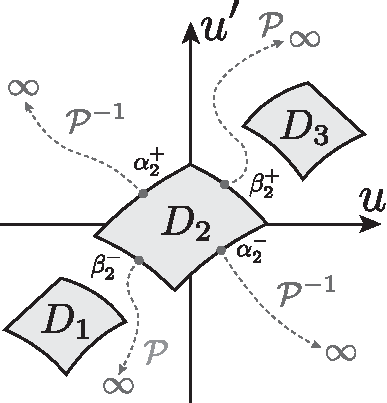
\includegraphics[scale = 1]{pic/island set}
	\caption{Hypothetical example of an island set $\mathcal{D} = \bigcup_{i \in \{1, 2, 3\}} D_i$ on a plane of initial conditions for equation \eqref{eq:stationary}. Boundaries of each component are mapped to the infinity by the $\mathcal{P}$ and $\mathcal{P}^{-1}$ maps (i.e. the corresponding solution of Cauchy problem collapses at $x = L$ and $x = -L$ respectively).}
\label{fig:islands-set}
\end{figure}

\subsection{Curves and Strips}

Move on to the definition of h,v-curves and h,v-strips.

\begin{definition}
	Let $D$ be an island bounded by curves $\alpha^{\pm}$, $\beta^{\pm}$.
	Consider a curve $\alpha$ that connects the opposite sides $\beta^{\pm}$ of the island $D$. 
	We call such curve as {\bf h-curve} (or $\mathrm{h}_{\gamma}$-curve) if it represents a graph of a monotonic $\gamma$-Lipschitz function $u' = h(u)$ and its monotonicity type coincides with the functions $u' = h_{\pm}(u)$ that correspond to the $\alpha^{\pm}$ boundaries of the island $D$.
	We also call {\bf h-strip} (or $\mathrm{h}_{\gamma}$-strip) an open subset of the island $D$ bounded by two $\mathrm{h}_{\gamma}$-curves.
\end{definition}

\begin{remark}
	We say that h-curve $\alpha$ is increasing / decreasing if it's a graph of increasing / decreasing function $u' = f(u)$.
\end{remark}

\begin{definition}
	Similarly consider a curve $\beta$ that connects opposite sides $\alpha^{\pm}$ of an island $D$.
	We call it as {\bf v-curve} (or $\mathrm{v}_{\gamma}$-curve) if it represents a graph of a monotonic $\gamma$-Lipschitz function $u = v(u')$ and its monotonicity type coincide with the functions $u = v_{\pm}(u')$ that correspond to the $\beta^{\pm}$ boundaries of the island $D$.
	Also we call {\bf v-strip} (or $\mathrm{v}_{\gamma}$-strip) an open subset of the island $D$ bounded by two $\mathrm{v}_{\gamma}$-curves.
\end{definition}

\begin{remark}
	We say that a v-curve $\beta$ is increasing / decreasing if it's a graph of increasing / decreasing function $u = f(u')$.
\end{remark}

\begin{remark}
	Island by itself represents a limit case of the h and v strips simultaneously.
\end{remark}

% TODO: Make this figure a bit smaller, use 16 pt. for letters.
\begin{figure}[h]
\centering
	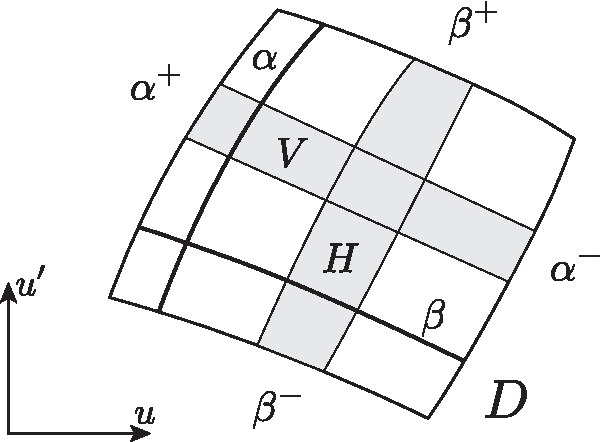
\includegraphics[scale = 1]{pic/curves and strips}
	\caption{An island $D$ bounded by curves $\alpha^{\pm}$, $\beta^{\pm}$; h-curve $\alpha$, v-curve $\beta$, and two strips: h-strip $H$ and v-strip $V$.}
\label{fig:curves-and-strips}
\end{figure}

All the above introduced definitions are illustrated in Figures \ref{fig:islands-set} and \ref{fig:curves-and-strips}.
At last let's define one additional property of island set along with $\mathcal{P}$, $\mathcal{P}^{-1}$ maps.

\begin{definition}
	Let $\mathcal{D}$ be an island set that is a domain for both $\mathcal{P}$ and $\mathcal{P}^{-1}$ maps.
	Consider two islands $D_1, D_2 \in \mathcal{D}$.
	We call the island $D_2$ {\bf forward-reachable} from the island $D_1$ if for any \emph{h}-curve $\alpha \in D_1$ with endpoints lying on the opposite boundaries $\beta_1^{\pm}$ of the island $D_1$ the intersection $\mathcal{P}(\alpha) \cap D_2$ is not empty.
	On the other hand we call the island $D_2$ {\bf backward-reachable} from the island $D_1$ if for any \emph{v}-curve $\beta \in D_1$ with endpoints lying on the opposite boundaries $\alpha_1^{\pm}$ of the island $D_1$ the intersection $\mathcal{P}^{-1}(\beta) \cap D_2$ is not empty.
	Finally we call the island $D_2$ {\bf reachable} from the $D_1$ if it satisfies both forward and backward reachability.
\end{definition}

\begin{remark}
	If an island $D_2$ is forward-reachable from $D_1$ then $D_1$ is backward-reachable from $D_2$ and vice versa.
\end{remark}

\begin{definition}
	We call an island set $\mathcal{D} = \bigcup_{i \in S} D_i$ {\bf complete} if for any $i, j$ island $D_i$ is reachable from $D_j$.
\label{def:complete-island-set}
\end{definition}

\subsection{Thickness of Strips}

Next we'll also need a definition of the strips thickness.
Let an h-strip $H$ lie inside an island $D$ and is bounded by h-curves $\alpha^+$ and $\alpha^-$.
Consider graphs of these curves as functions of $u$: $u' = h_{\pm}(u)$.
By definition, $h_{\pm}(u)$ are $\gamma$-Lipschitz functions.
Denote their domains by $\Delta^{\pm}$.
Due to the geometric properties of an island, domains $\Delta^{\pm}$ do not coincide except the case when the opposite boundaries of the island $D$ are vertical straight lines.
Let $\Delta^+ = [u_0^+; u_1^+]$, $\Delta^- = [u_0^-; u_1^-]$, consider new domain $\Delta = \Delta^+ \cup \Delta^-$ and define functions $\widetilde{h}_{\pm}(u)$ on $\Delta$ as follows:
\begin{equation}
	\widetilde{h}_{\pm}(u) = \begin{cases}
		h_{\pm}(u_0^{\pm}) & u < u_0^{\pm}; \\
		h_{\pm}(u) & u \in \Delta^{\pm}; \\
		h_{\pm}(u_1^{\pm}) & u > u_1^{\pm}.
	\end{cases}
\label{eq:continuation}
\end{equation}
Since $h_{\pm}$ are $\gamma$-Lipschitz functions the new functions $\widetilde{h}_{\pm}$ are also $\gamma$-Lipschitz on the whole domain $\Delta$.
Denote by $\widetilde{\alpha}^{\pm}$ the curves that are the graphs of $\widetilde{h}_{\pm}(u)$.

\begin{definition}
\label{def:h-thickness}
	By {\bf thickness} of an \emph{h}-strip $H$, denoted $d_\emph{h}(H)$, we mean the distance between curves $\widetilde{\alpha}^{\pm}$ in C-norm, i.e.
	\begin{equation}
		d_\emph{h}(H) = d(\widetilde{\alpha}^+, \widetilde{\alpha}^-) = \max \limits_{u \in \Delta} |\widetilde{h}_+(u) - \widetilde{h}_-(u)|.
	\label{eq:h-thickness}
	\end{equation}
\end{definition}

\begin{remark}
\label{remark:h-strips-thickness}
	For two \emph{h}-strips $H_1$, $H_2$ the following statement is valid: $H_2 \subseteq H_1 \Rightarrow \Delta_2 \subseteq \Delta_1$ and $d_\emph{h}(H_2) \le d_\emph{h}(H_1)$.
\end{remark}

\begin{definition}
	Let maximum of the expression \eqref{eq:h-thickness} be reached at point $u_*$, i.e.
	\begin{equation}
		u_* = \argmax \limits_{u \in \Delta} |\widetilde{h}_+(u) - \widetilde{h}_-(u)|.
	\label{eq:argmax}
	\end{equation}
	We call \emph{h}-strip $H$ {\bf well-measurable} if $u_* \in \Delta^+ \cap \Delta^-$.
\label{def:well-measurable-h-strip}
\end{definition}

\begin{figure}[h]
\centering
	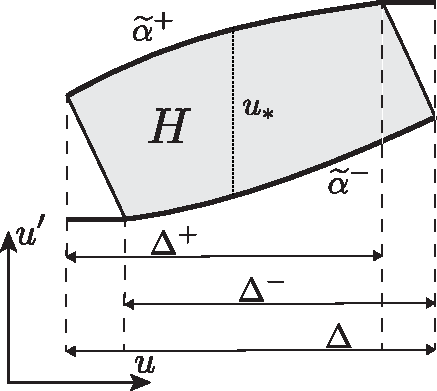
\includegraphics[scale = 1]{pic/thickness definition}
	\caption{An illustration to the definition of an h-strip thickness. Strip $H$ is {\it well-measurable} in a sense of Definition \ref{def:well-measurable-h-strip}. Curves $\widetilde{\alpha}^{\pm}$ are continuations of the initial h-strip borders to the whole $\Delta$; $u_*$ is a point of maximum of the expression \eqref{eq:h-thickness}.}
\label{fig:thickness-definition}
\end{figure}

\begin{proposition}
\label{prop:h-strip-domains}
	For \emph{h}-strip $H$ the following statement is valid:
	\begin{equation}
		\Delta^+ \cap \Delta^- \neq \varnothing \Rightarrow u_* \in \Delta^+ \cap \Delta^-,
	\end{equation}
	i.e. \emph{h}-strip is well-measurable if domains of its border functions have at least one common point.
\end{proposition}
\begin{proof}
	The statement immediately follows from the monotonicity of the h-strip borders $\alpha^+$ and $\alpha^-$.
\end{proof}

In a similar way we define thickness of v-strips.
Let an v-strip $V$ lie inside an island $D$ and is bounded by v-curves $\beta^+$ and $\beta^-$.
Consider this curves as a functions of $u'$: $u = v_{\pm}(u')$.
Denote domains of these functions by $\Delta^{\pm}$.
Continue functions $v_{\pm}(u')$ to the whole interval $\Delta = \Delta^+ \cap \Delta^-$ in the same way as for h-strips, see \eqref{eq:continuation}, and introduce new functions $\widetilde{v}_{\pm}(u')$ and curves $\widetilde{\beta}^{\pm}$.

\begin{definition}
\label{def:v-thickness}
	By {\bf thickness} of an \emph{v}-strip $V$, denoted $d_\emph{v}(V)$, we mean the distance between curves $\widetilde{\beta}^{\pm}$ in C-norm, i.e.
	\begin{equation}
		d_\emph{v}(V) = d(\widetilde{\beta}^+, \widetilde{\beta}^-) = \max \limits_{u' \in \Delta} |\widetilde{v}_+(u') - \widetilde{v}_-(u')|.
	\label{eq:v-thickness}
	\end{equation}
\end{definition}

The definition of {\it well-measurable} v-strip is introduced in a same way.
Remark~\ref{remark:h-strips-thickness} and Proposition~\ref{prop:h-strip-domains} can be also written for v-strips.
Note that thickness of h-strip is measured in vertical direction, and thickness of v-strip is measured in horizontal direction.
If a strip is well-measurable then its thickness is measured in a direction along the straight line that connects points from the opposite side of the strip.

\section{Poincar\'e Map Domains for Piecewise Periodic Pseudopotential}
\label{section:poincare-map-domains-piecewise}

Let's demonstrate how the definitions introduced above work all together.
For that purpose consider equation \eqref{eq:stationary} with $Q(x) \equiv -1$ and periodic piecewise constant pseudopotential $P(x) = \eta(x)$, where $\eta(x)$ is a function of the period $L = L_* + L_0$, defined as
\begin{equation}
	\eta(x) = \left\{
		\begin{array}{rl}
			-1, & x \in [0; L_*); \\
			+1, & x \in [L_*; L_* + L_0),
		\end{array}
	\right.
\label{eq:eta}
\end{equation}
Function \eqref{eq:eta} is represented in Figure~\ref{fig:piecewise-constant}.
Equation \eqref{eq:stationary} takes form
\begin{equation}
	u_{xx} - u + \eta(x) u^3 = 0. 
\label{eq:stationary-piecewise}
\end{equation}
% TODO: This is not a function! Fix it!
\begin{figure}[h]
\centering
	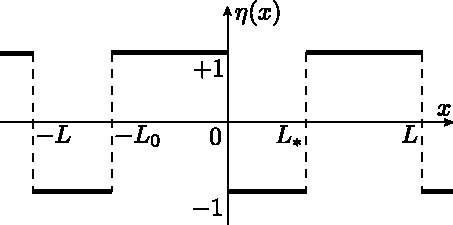
\includegraphics[scale = 1.2]{pic/piecewise constant}
	\caption{Plot of function $\eta(x)$ defined in \eqref{eq:eta}.}
\label{fig:piecewise-constant}
\end{figure}
Since pseudopotential is a piecewise constant function that has only two different values on the period $L$ we can split the period into two intervals and consider two different cases for equation \eqref{eq:stationary-piecewise}.
In each region Eq.~\eqref{eq:stationary-piecewise} has a form of conservative Duffing equation:
\begin{eqnarray}
	&& u_{xx} - u - u^3 = 0, \quad x \in [0; L_*];\label{eq:stationary-piecewise-singular} \\
	&& u_{xx} - u + u^3 = 0, \quad x \in [L_*; L_* + L_0] \label{eq:stationary-piecewise-regular}.
\end{eqnarray}
Each of equations \eqref{eq:stationary-piecewise-singular}, \eqref{eq:stationary-piecewise-regular} can be solved explicitly  through Jacobi elliptic functions.
Exact solutions are given in Appendix \ref{appendix:solutions-of-duffing-equations}.
\begin{figure}[h]
\centering
	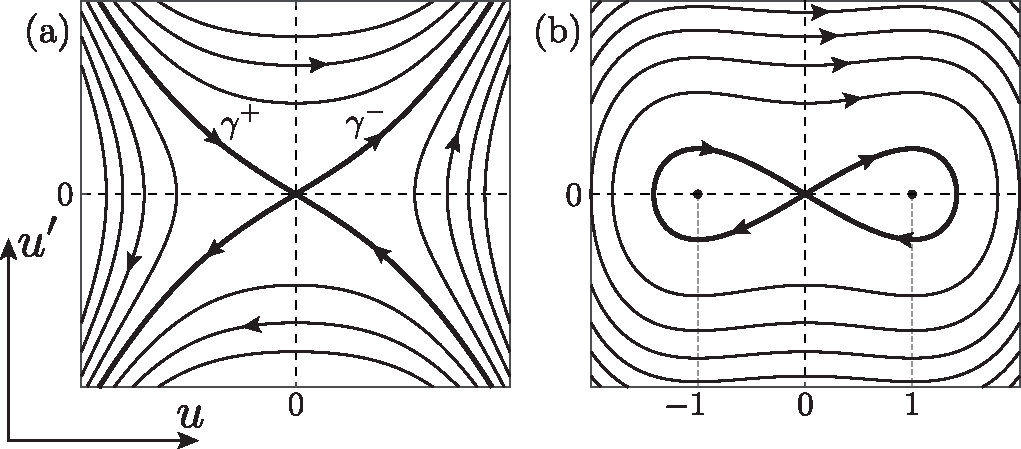
\includegraphics[scale = 1]{pic/phase portraits}
	\caption{Phase portraits for different cases of equation \eqref{eq:stationary-piecewise} with piecewise pseudopotential \eqref{eq:eta}. Panel (a) represents the phase portrait for equation \eqref{eq:stationary-piecewise-singular}, curves $\gamma^{\pm}$ correspond to the separatrices which enter the equilibrium point $(0, 0)$ as $x$ approaches $\pm \infty$. Panel (b) depicts the phase portrait for equation \eqref{eq:stationary-piecewise-regular}.}
\label{fig:phase-portraits}
\end{figure}

Equation \eqref{eq:stationary-piecewise-singular} has a first integral of the form:
\begin{equation}
	H_* = u_x^2 - u^2 - \frac{1}{2} u^4.
\label{eq:stationary-piecewise-singular-integral}
\end{equation}
The phase portrait for equation \eqref{eq:stationary-piecewise-singular} is presented in Figure \ref{fig:phase-portraits} (a).
Any trajectory on the phase plane corresponds to some value of $H_*$.
Level $H_* = 0$ corresponds to the equilibrium state $(0, 0)$, and four separatrices related to it.
Two of the separatrices $\gamma_{1,2}^+$ enter the zero equilibrium as $x$ approaches $+\infty$.
We denote them by curve $\gamma^+$.
Another two separatrices $\gamma_{1,2}^-$ enter the zero equilibrium as $x$ approaches $-\infty$.
We denote them by curve $\gamma^-$ correspondingly.
Resulting curves $\gamma^{\pm}$ satisfy the equations
\begin{equation}
	u' = \pm \frac{u}{\sqrt{2}} \sqrt{2 + u^2}.
\end{equation}

It follows from the exact form of the solutions of equation \eqref{eq:stationary-piecewise-singular} that all of them, except the zero one, are singular.
It means that a solution for a Cauchy problem with initial conditions $u(0) = u_0$, $u'(0) = u_0'$ ($u_0$ and $u_0'$ not equals zero simultaneously) tends to infinity while $x$ approaches some finite point both to the left and to the right of $x = 0$.
It means that a solution for equation \eqref{eq:stationary-piecewise-singular} has a {\it finite domain} if $H_* \neq 0$.

The first integral of equation \eqref{eq:stationary-piecewise-regular} is
% TODO: Consider to use (u')^2 instead of (u_x)^2.
\begin{equation}
	H_0 = u_x^2 - u^2 + \frac{1}{2} u^4.
\label{eq:stationary-piecewise-regular-integral}
\end{equation}
Phase portrait for equation \eqref{eq:stationary-piecewise-regular} is given in Figure \ref{fig:phase-portraits} (b).
It has two center equilibrium points $(\pm 1, 0)$ and one hyperbolic equilibrium point $(0, 0)$.
Separatrix loops correspond to the localized solutions
\begin{equation}
	u(x) = \pm \frac{\sqrt{2}}{\cosh{x}}.
\end{equation}
The area inside the separatrix loops is filled by closed orbits of periodic solutions with nonzero mean.
All other orbits turn around the origin and correspond to solutions with zero mean.
That's why we mark a corresponding period part $L_0$ with a symbol ``$0$'', since it looks like a little curve circle.

\subsection{General Propositions on the $\mathscr{U}_L^{\pm}$ Sets for Piecewise Pseudopotential}

Let's move on to the consideration of the $\mathscr{U}_L^{\pm}$ sets for equation \eqref{eq:stationary-piecewise}.
We consider a decomposition of the Poincar\'e map $\mathcal{P} = \mathcal{P}_0 \mathcal{P}_*$, where  maps associated with corresponding parts of the overall period $L$ are defined in a similar manner as the initial Poincar\'e map $\mathcal{P}$ itself \eqref{eq:poincare-map}.
Map $\mathcal{P}_*$ maps a point $(u_0, u_0')$ to $(u(L_*), u'(L_*))$ where $u(x), \, x \in [0; L_*]$ is a solution of Eq.~\eqref{eq:stationary-piecewise-singular} with initial conditions $u(0) = u_0$, $u'(0) = u_0'$.
Similarly map $\mathcal{P}_0$ maps a point $(u_0, u_0')$ to $(u(L), u'(L))$ where $u(x), \, x \in [L_*; L]$ is a solution of Eq.~\eqref{eq:stationary-piecewise-regular} with initial conditions $u(L_*) = u_0$, $u'(L_*) = u_0'$.

Note that $\mathcal{P}_*$ is not defined in the whole $\mathbb{R}^2$.
We denote by $\mathscr{U}_{L_*}^+$ a domain of the map $\mathcal{P}_*$.
Due to the fact that all solutions of equation \eqref{eq:stationary-piecewise-regular} are regular, domain of the map $\mathcal{P}$ coincide with the domain of $\mathcal{P}_*$ map, i.e.
\begin{equation}
	\mathscr{U}_L^+ = \textrm{dom}(\mathcal{P}) = \textrm{dom}(\mathcal{P}_0 \mathcal{P}_*) = \textrm{dom}(\mathcal{P}_*) \equiv \mathscr{U}_{L_*}^+.
\end{equation}

Since the phase portrait for Eq.~\eqref{eq:stationary-piecewise-singular} is symmetric with respect to the origin, $\mathscr{U}_{L_*}^+$ is also symmetric with respect to the origin (see how its computed in Figure \ref{fig:poincare-map-domain-piecewise}).
Two separatrices $\gamma_{1,2^+}$ that correspond to the curve $\gamma^+$ enter zero equilibrium as $x \to +\infty$.
It means that for any initial data posed at $\gamma^+$ and for any $L_*$ the map $\mathcal{P}_*$ is correctly defined, i.e. $\gamma^+ \in \mathscr{U}_{L_*}^+$.
Another property of $\mathscr{U}_{L_*}^+$ directly follows from Proposition \ref{prop:domain-reflection}:
\begin{equation}
	\mathcal{P}_*(\mathscr{U}_{L_*}^+) = I (\mathscr{U}_{L_*}^+) = \mathscr{U}_{L_*}^-.
\label{eq:domain-reflection-singular-forward}
\end{equation}
% TODO: A comprehensive theorem can be added here.
%   1. Borders of $\mathscr{U}_{L_*}^+$ are decreasing curves.
%   2. Distance between borders tends to zero as $u \to \infty$, $u' \to \infty$.

Move on to the $\mathscr{U}_{L_*}^-$ set for equation \eqref{eq:stationary-piecewise-singular}.
Since $\mathscr{U}_{L_*}^-$ is a reflection of $\mathscr{U}_{L_*}^+$ with respect to the $u'$ axis, it inherits its symmetry properties.
Set $\mathscr{U}_{L_*}^-$ also contains curve $\gamma^-$ that corresponds to another two separatrices $\gamma_{1,2}^-$ of equation \eqref{eq:stationary-piecewise-singular}.
% TODO: A comprehensive theorem can be added here.
%   1. Borders of $\mathscr{U}_{L_*}^-$ are decreasing curves.
%   2. Distance between borders tends to zero as $u \to \infty$, $u' \to \infty$.
Consider the second map $\mathcal{P}_0$ of the decomposition.
As we mentioned above $\mathcal{P}_0$ is correctly defined on the whole $\mathscr{U}_{L_*}^-$.
It turns out that the image $\mathcal{P}_0(\gamma^-)$ has a spiral-like structure and intersects the curve $\gamma^+$ infinitely many times.
The following proposition is valid.

% TODO: Consider to use $\mathcal{O}(n^{-1})$ instead of $\mathcal{O}(H^{\nicefrac{-1}{4}})$.
\begin{proposition}
	$\mathcal{P}_0$-image of the curve $\gamma^-$ intersects $\gamma^+$ infinitely many times at the points $\{ 0 \} \cup {u_{\pm n}}$,
	\begin{equation}
		u_{\pm n} = \pm \frac{2 x_{n-1}}{\sqrt[4]{2} L_0} + \mathcal{O} \left( H_0^{\nicefrac{-1}{4}} \right), \ n \in \mathbb{N},
	\label{eq:separatrix-map-un}
	\end{equation}
	as $H_0 \to \infty$, where
	\begin{equation}
		x_n = \cn^{-1} \left( 2^{\nicefrac{-1}{4}}, k_0 \right) + K(k_0) n.
	\label{eq:separatrix-map-xn}
	\end{equation}
	Here $K(k)$ is the complete elliptic integral of the first kind, and $k_0 = 1 / \sqrt{2}$. 
\label{prop:separatrix-map}
\end{proposition}
\begin{proof}
	First of all, the point $(0, 0)$ belongs to the intersection $\mathcal{P}_0(\gamma^-) \cap \gamma^+$ since it's a stable fixed point of equation \eqref{eq:stationary-piecewise-regular} and the $\mathcal{P}_0$ map.

	Next we note that all the intersections $\mathcal{P}_0(\gamma^-) \cap \gamma^+$ occur outside of the separatrix loops of \eqref{eq:stationary-piecewise-regular} and correspond to zero mean solutions of \eqref{eq:stationary-piecewise-regular}.
	This obviously follows from that fact that $\gamma^+$ lies outside of the loops both from left and right of $u'$ axis (depicted in Fig.~\ref{fig:separatrix-map}~(a)).
	\begin{figure}[h]
	\centering
		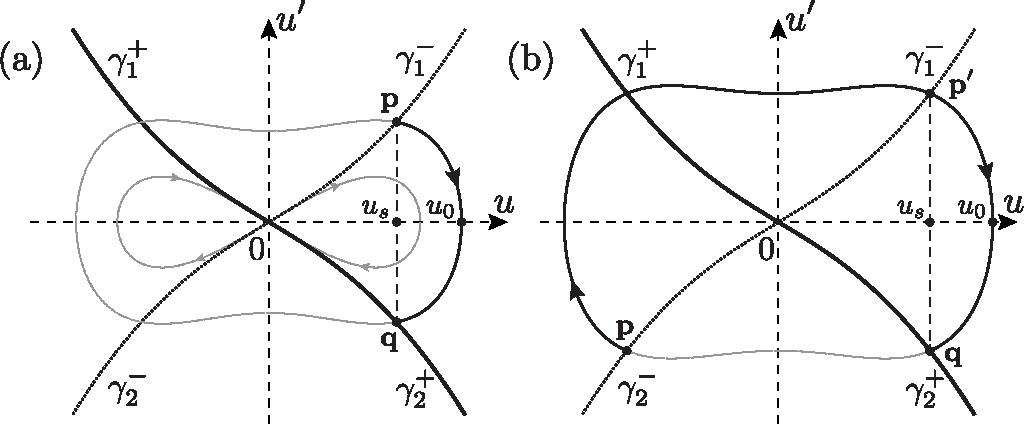
\includegraphics[scale = 1]{pic/separatrix map}
		\caption{Illustration to the proof of Proposition~\ref{prop:separatrix-map}.}
	\label{fig:separatrix-map}
	\end{figure}
	
	Prove the formula for the points from the right side of $u'$ axis, $u_{+n}$.
	Such points corresponds to the $\gamma_2^+$ separatrix of equation \eqref{eq:stationary-piecewise-singular}, see Figure~\ref{fig:separatrix-map}.
	Result points of intersections $\mathcal{P}_0(\gamma^-) \cap \gamma_2^+$ can be divided into two groups: $\mathcal{P}_0(\gamma_1^-) \cap \gamma_2^+$ and $\mathcal{P}_0(\gamma_2^-) \cap \gamma_2^+$.

	Consider points from the first group.
	Let a point $\vb{q}$ belong to the intersection $\mathcal{P}_0(\gamma_1^-) \cap \gamma_2^+$.
	Then there exists a point $\vb{p} = (u_s, u_s') \in \gamma_1^-$ such that $\mathcal{P}_0(\vb{p}) \in \gamma_2^+$.
	Due to the symmetries of the phase portraits for equations \eqref{eq:stationary-piecewise-singular} and \eqref{eq:stationary-piecewise-regular}, $\vb{q} = (u_s, -u_s')$, see Figure~\ref{fig:separatrix-map}~(a).
	Consider a phase trajectory of \eqref{eq:stationary-piecewise-regular} that lies outside of separatrix loop and connects points $\vb{p}$ and $\vb{q}$.
	According to Appendix~\ref{appendix:solutions-of-duffing-equations} exact form of the solution is
	\begin{equation}
		u(x) = x_0 \cn \left( \sqrt{x_0^2 - 1} x + x_1, k \right),
	\label{eq:stationary-piecewise-regular-solution}
	\end{equation}
	where $k$ is elliptic modulus,
	\begin{equation}
		k = \dfrac{1}{\sqrt{2}} \dfrac{x_0}{\sqrt{x_0^2 - 1}},
	\end{equation}
	and $x_0$, $x_1$ are constants that are determined by initial conditions $(u(0), u'(0)) = \vb{p}$.
	
	Next let's introduce $x$ variable shift $x \to x - L_0 / 2$.
	Equation \eqref{eq:stationary-piecewise-regular-solution} persists its form but now $u(0) = u_0, \ u_0 > 0$, and $u'(0) = 0$.
	That allows us to determine constants $x_0, \, x_1$: $x_0 = u_0,$ $x_1 = 0$.
	Solution \eqref{eq:stationary-piecewise-regular-solution} takes form
	\begin{equation}
		u(x) = u_0 \cn \left( \sqrt{u_0^2 - 1} x, k \right),
	\label{eq:stationary-piecewise-regular-solution-shifted}
	\end{equation}
	and for coordinates of the points $\vb{p}$ and $\vb{q}$ we have
	\begin{alignat}{3}
		& \vb{p} = (u(-L_0 / 2), && \ u'(-L_0 / 2)) && = (u_s, u_s'); \label{eq:p-first-group} \\
		& \vb{q} = (u(L_0 / 2),  && \ u'(L_0 / 2)) && = (u_s, -u_s'). \label{eq:q-first-group}
    \end{alignat}
	Since value of $H_0$ \eqref{eq:stationary-piecewise-regular-integral} conserves on the trajectory that connects point $\vb{p}$ and the point $(u_0, 0)$ one can write
	\begin{equation}
		H_0 = -u_0^2 + \frac{u_0^4}{2} = (u_s')^2 - u_s^2 + \frac{u_s^4}{2}.
	\label{eq:trajectory-H0}
	\end{equation}
	On the other hand the point $\vb{p}$ belong to the separatrix of \eqref{eq:stationary-piecewise-singular} and its coordinates satisfy an equality
	\begin{equation}
		H_* = (u_s')^2 - u_s^2 - \frac{u_s^4}{2} = 0.
	\label{eq:separatrix-H*}
	\end{equation}
	Comparing \eqref{eq:trajectory-H0} and \eqref{eq:separatrix-H*} one can conclude that
	\begin{equation}
		u_s^4 = \frac{u_0^4}{2} - u_0^2.
	\label{eq:separatrix-u-coordinate}
	\end{equation}
	At the point $\vb{q}$ we have
	\begin{equation}
		u_s = u_0 \cn \left(\frac{\sqrt{u_0^2 - 1} L_0}{2}, k \right).
	\label{eq:stationary-piecewise-regular-solution-q}
	\end{equation}
	Substitute $u_s$ from \eqref{eq:separatrix-u-coordinate} into \eqref{eq:stationary-piecewise-regular-solution-q}, divide both side of the equality by $u_0$, and introduce $4 v_0^2 = u_0^2 - 1$.
	Equation \eqref{eq:stationary-piecewise-regular-solution-q} takes form
	\begin{equation}
		\left( \frac{1}{2} - \frac{1}{4 v_0^2 + 1} \right)^{1/4} = \cn \left( v_0 L_0, k \right), \quad k = \frac{1}{\sqrt{2}} \sqrt{1 + \frac{1}{4 v_0^2}}.
	\label{eq:v0-elliptic-relation}
	\end{equation}
	
	Let us analyse the limit $v_0 \to \infty$.
	First of all consider $k$ as a function of $v_0$ and expand it into the series:
	\begin{equation}
		k(v_0) = \frac{1}{\sqrt{2}} + \frac{1}{8 \sqrt{2}} \frac{1}{v_0^2} - \frac{1}{32 \sqrt{2}} \frac{1}{v_0^4} + \dots.
	\label{eq:k-series}
	\end{equation}
	Let $k_0 = 1/\sqrt{2}$.
	We introduce the remainder $\Delta k = k(v_0) - k_0$.
	Note that $\Delta k$ has the main term of order $v_0^{-2}$ as $v_0 \to \infty$.
	Denote $w_0 = v_0 L_0$, consider $\cn(w_0, k)$ in the right side of \eqref{eq:v0-elliptic-relation} as a function of elliptic modulus $k$ and expand it into the series in the vicinity of $k_0$ up to the second term:
	\begin{equation}
		\cn \left( w_0, k_0 + \Delta k \right) = \cn \left( w_0, k_0 \right) + f(w_0, k_0) \Delta k + \mathcal{O}(w_0^{-1/4}).
	\label{eq:elliptic-cosine-expansion}
	\end{equation}
	Here $f(w_0, k_0)$ is the first derivative of elliptic cosine with respect to $k$ at $k = k_0$:
	% TODO: Give a link to Abramowitz and Stegun.
	\begin{equation}
		f(w_0, k_0) = \frac{\sn (w_0) \dn (w_0) (w_0 - k_0 w_0 + k_0 \sn(w_0) \cd(w_0) - E(\phi(w_0))) }{2 (k_0 - 1) k_0} .
	\end{equation}
	Here $\phi(w, k)$ is the Jacobi amplitude and $E(\phi, k)$ is the incomplete elliptic integral of the second kind.
	All elliptic functions have the same modulus $k_0$, we omit this parameter for the sake of brevity.
	This expression is quite tremendous, nevertheless, what interests us here is the orders of terms with respect to $w_0$.
	It has a leading term of order $w_0$ as $w_0 \to \infty$.
	That allows us to conclude that the term $f(w_0, k_0) \Delta k$ of \eqref{eq:elliptic-cosine-expansion} in its turn has a leading term of order $w_0^{-1}$ (or $v_0^{-1}$).
	Rewrite \eqref{eq:v0-elliptic-relation} in a form:
	\begin{equation}
		\left( \frac{1}{2} - \frac{1}{4 v_0^2 + 1} \right)^{1/4} = \cn \left( v_0 L_0, k_0 \right) + \mathcal{O}(v_0^{-1}),
	\label{eq:v0-elliptic-relation-asymptotic}
	\end{equation}
	Using the same approach again we expand the left side of \eqref{eq:v0-elliptic-relation-asymptotic} into a series:
	\begin{equation}
		\left( \frac{1}{2} - \frac{1}{4 v_0^2 + 1} \right)^{1/4} =  \frac{1}{\sqrt[4]{2}} - \frac{1}{2 \sqrt[4]{2}} \frac{1}{(4v_0^2 + 1)} + \mathcal{O}(v_0^{-4}).
	\label{eq:v0-elliptic-relation-left-side-expansion}
	\end{equation}
	Combining \eqref{eq:v0-elliptic-relation-left-side-expansion} with \eqref{eq:v0-elliptic-relation-asymptotic} and comparing the orders of terms we conclude that
	\begin{equation}
		\cn (v_0 L_0, k_0) = \frac{1}{\sqrt[4]{2}} + \mathcal{O}(v_0^{-1}).
	\end{equation}
	Let's express $v_0 L_0$ in the equation above 
	\begin{equation}
		v_0 L_0 = \cn^{-1} \left( \frac{1}{\sqrt[4]{2}} + \mathcal{O}(v_0^{-1}), k_0 \right) + 2 K(k_0) n, \quad n \in \{0\} \cup \mathbb{N}.
	\label{eq:v0-L0-expression}
	\end{equation}
	Here $K(k)$ is the complete elliptic integral of the first kind. 
	We left only positive roots since we are interested only in intersections $\mathcal{P}_0(\gamma_1^-) \cap \gamma_2^+$ where $u_0$ is positive and we can write
	\begin{equation}
		v_0 = \frac{u_0}{2} \sqrt{1 - \frac{1}{u_0^2}} = \frac{u_0}{2} - \frac{1}{2u_0} + \mathcal{O}(u_0^{-3}).
	\label{eq:v0-through-u0}
	\end{equation}
	We note that by definition of $\cn^{-1}$ function
	\begin{equation}
		\cn^{-1} \left( 2^{\nicefrac{-1}{4}} + \mathcal{O}(v_0^{-1}) \right) = F \left( \arccos \left( 2^{\nicefrac{-1}{4}} + \mathcal{O}(v_0^{-1}) \right), k_0 \right),
	\label{eq:inverse-elliptic-cosine-definition}
	\end{equation}
	where $F(\phi, k)$ is incomplete elliptic integral of the first kind.
	Consider series expansion of $\arccos$ up to the main term:
	\begin{equation}
		\arccos \left( 2^{\nicefrac{-1}{4}} + \mathcal{O}(v_0^{-1}) \right) = \arccos \left( 2^{\nicefrac{-1}{4}} \right) + \mathcal{O}(v_0^{-1}).
	\label{eq:arccos-expansion}
	\end{equation}
	Let's substitute \eqref{eq:arccos-expansion} into \eqref{eq:inverse-elliptic-cosine-definition}, use additive property of integral, and apply integral mean value theorem to the second term:
	\begin{equation}
	\begin{split}
		\cn^{-1} \left( 2^{\nicefrac{-1}{4}} + \mathcal{O}(v_0^{-1}) \right) & = F \left( \arccos \left( 2^{\nicefrac{-1}{4}} \right) + \mathcal{O}(v_0^{-1}), k_0 \right) = \\ & = F \left( \arccos \left( 2^{\nicefrac{-1}{4}} \right), k_0 \right) + F \left( \mathcal{O}(v_0^{-1}), k_0 \right) = \\ & = \cn^{-1} \left( 2^{\nicefrac{-1}{4}}, k_0 \right) + \mathcal{O}(v_0^{-1}).
	\end{split}
	\label{eq:inverse-elliptic-cosine-asymptotic}
	\end{equation}
	Put \eqref{eq:inverse-elliptic-cosine-asymptotic} and \eqref{eq:v0-through-u0} into \eqref{eq:v0-L0-expression}, also note that according to \eqref{eq:v0-through-u0} we can safely replace $\mathcal{O}(v_0^{-1})$ with $\mathcal{O}(u_0^{-1})$,
	\begin{equation}
		u_0 = \frac{2}{L_0} \left( \cn^{-1} \left( 2^{\nicefrac{-1}{4}}, k_0 \right) + 2 K(k_0) n \right) + \mathcal{O}(u_0^{-1}).
	\label{eq:u0-expression}
	\end{equation}
	Finally let's get rid of $u_0$ in favor of $u_s$.
	For that purpose according to \eqref{eq:trajectory-H0} we can write $\mathcal{O}\left(H_0^{\nicefrac{-1}{4}}\right)$ instead of $\mathcal{O}(u_0^{-1})$, and it follows from \eqref{eq:separatrix-u-coordinate} that
	\begin{equation}
		u_s = \dfrac{1}{\sqrt[4]{2}} u_0 + \mathcal{O}(u_0^{-1}).	
	\end{equation}
	Let's introduce the following denotation
	\begin{equation}
		x_n = \cn^{-1} \left( 2^{\nicefrac{-1}{4}}, k_0 \right) + 2K(k_0)n.
	\label{eq:xn-first-group}
	\end{equation}
	Now combining the expressions above all together and replacing $u_s$ with $u_{+n}$ we get
	\begin{equation}
		u_{+n} = \frac{2 x_{n-1}}{\sqrt[4]{2} L_0} + \mathcal{O} \left( H_0^{\nicefrac{-1}{4}} \right), \quad n \in \mathbb{N}.
	\label{eq:un-final-positive}
	\end{equation}
	
	In order to get the final formula of the proposition for $\{ u_{+n} \}$ we need to consider points of intersections from the second group $\mathcal{P}_0 (\gamma_2^-) \cap \gamma_2^+$.
	We can easily reduce this task to the previous one.
	Let there exists a point of intersection $\vb{q} \in \gamma_2^+$. 
	Consider point $\vb{p} \in \gamma_2^-$, such that $\mathcal{P}_0(\vb{p}) = \vb{q}$, see Fig.~\ref{fig:separatrix-map}~(b).
	We note that there exists a point $\vb{p}' \in \gamma_1^-$, and the trajectory \eqref{eq:stationary-piecewise-regular-solution} goes from the point $\vb{p}$ to $\vb{p}'$ over a half of the period $2K(k) / \sqrt{x_0^2 - 1}$, and after that cross the $u$ axis at the point $u_0$.
	Then we introduce an $x$ variable shift $x \to x - (L_0 / 2 + K(k) / \sqrt{x_0^2 - 1})$, so that $u(0) = u_0, \ u_0 > 0$, and $u'(0) = 0$, and can determine $x_0 = u_0$, $x_1 = 0$.
	Solution \eqref{eq:stationary-piecewise-regular-solution} takes form \eqref{eq:stationary-piecewise-regular-solution-shifted} again and for coordinates of the points $\vb{p}'$ and $\vb{q}$ we have
	\begin{alignat}{4}
		& \vb{p}' && = \bigg( u \bigg( -L_0 / 2 + \tfrac{K(k)}{\sqrt{u_0^2 - 1}} \bigg), && \ u' \bigg( -L_0 / 2 + \tfrac{K(k)}{\sqrt{u_0^2 - 1}} \bigg) \bigg) && = (u_s, u_s'); \label{eq:p'-second-group} \\
		& \vb{q} && = \bigg( u \bigg(L_0 / 2 - \tfrac{K(k)}{\sqrt{u_0^2 - 1}} \bigg),  && \ u' \bigg( L_0 / 2 - \tfrac{K(k)}{\sqrt{u_0^2 - 1}} \bigg) \bigg) && = (u_s, -u_s'). \label{eq:q-second-group}
    \end{alignat}
    Now we can use relations \eqref{eq:p'-second-group}, \eqref{eq:q-second-group} instead of \eqref{eq:p-first-group}, \eqref{eq:q-first-group}, and repeat all the steps above.
    Difference in $x$ variable shift results in the additional term $K(k)$ in \eqref{eq:v0-L0-expression} and \eqref{eq:u0-expression}.
    Finally we replace $K(k) = K(k_0 + \Delta k) = K(k_0) + \mathcal{O}(H_0^{\nicefrac{-2}{4}})$, and get the following relation for $x_n$:
	\begin{equation}
		x_n = \cn^{-1} \left( 2^{\nicefrac{-1}{4}}, k_0 \right) + K(k_0) (2n + 1).
	\label{eq:xn-second-group}
	\end{equation}
	Relation \eqref{eq:un-final-positive} remains the same.
	Combining \eqref{eq:xn-first-group} with \eqref{eq:xn-second-group} we get the result for separatrix intersections points $\{ u_{+n} \} \in \mathcal{P}(\gamma^-) \cap \gamma_2^+$:
	\begin{equation}
		u_{+n} = \frac{2 x_{n-1}}{\sqrt[4]{2} L_0} + \mathcal{O} \left( H_0^{\nicefrac{-1}{4}} \right), \quad n \in \mathbb{N},
	\label{eq:us-final}
	\end{equation}
	where $x_n$ satisfies the relation
	\begin{equation}
		x_n = \cn^{-1} \left( 2^{\nicefrac{-1}{4}}, k_0 \right) + K(k_0) n.
	\label{eq:xn-final}
	\end{equation}
	
	Points $\{ u_{-n} \} , \ n \in \mathbb{N}$ from the left side of $u'$ axis, $u_{-n} \in \mathcal{P}_0(\gamma^-) \cap \gamma_1^+$, should be treated in a similar way, proposition is proven.
\end{proof}

Propositions~\ref{prop:separatrix-map} says that the far we goes from the $(0, 0)$ point on the phase plane, the better the asymptotic relation \eqref{eq:separatrix-map-un} works.
It turns out that formula \eqref{eq:separatrix-map-un} works pretty well even for small number of $n$.
See Figure~\ref{fig:separatrix-map-with-numerical-computations} where we compare the predicted coordinates with actual intersections obtained by numerical computation of $\mathcal{P}_0(\gamma^-)$.
Another interesting consequence of Proposition~\ref{prop:separatrix-map} is that set $\mathscr{U}_{L}$ consists of infinitely many connected components.
This obviously follows from that fact, that set $\mathscr{U}_{L_*}^-$ contains the entire curve $\gamma^-$ and map $\mathcal{P}_0$ is continuous, so the image $\mathcal{P}_0 (\mathscr{U}_{L_*}^-)$ cross $\mathscr{U}_{L}^+$ infinitely many times.
\begin{figure}[h]
\centering
	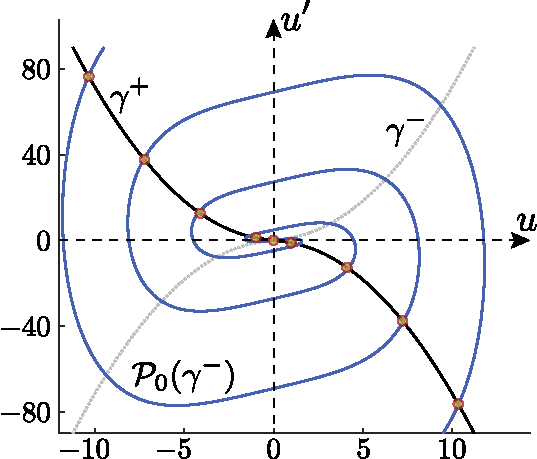
\includegraphics[scale = 1]{pic/separatrix map with numerical computations}
	\caption{
		Comparison of asymptotic formula \eqref{eq:separatrix-map-un} with numerical computations for $L_0 = 1$.
		Curves $\gamma^{\pm}$ are formed by the separatrices of \eqref{eq:stationary-piecewise-singular}, $\mathcal{P}_0$-image of $\gamma^-$ is a solid blue line computed numerically.
		Predicted points of intersections $u_{\pm n}$ from $\mathcal{P}_0(\gamma^-) \cap \gamma^+$ are marked with yellow dots. One can see that \eqref{eq:separatrix-map-un} predicts intersections quite precisely even for small number of $n$.
	}
\label{fig:separatrix-map-with-numerical-computations}
\end{figure}

\subsection{Construction of the Poincar\'e Map Domains}

One of the possible way to construct $\mathscr{U}_L^{\pm}$ sets for different maps associated with equation \eqref{eq:stationary} is to use a numerical procedure called scanning of initial conditions plane $(u, u')$.
That's how it works.
At first ranges of scanning $u_{\min} \le u \le u_{\max}$, $u_{\min}' \le u' \le u_{\max}'$ are selected.
Then the target segment of the initial conditions plane is covered by a uniform grid with small steps $h$ and $h'$ for each axis $u$ and $u'$.
Using Runge-Kutta 4th order method we solve differential equation in each node of the resulting grid.
We use an interval $[0; L]$ for $\mathscr{U}_L^+$ where $x$ changes in forward direction from $0$ to $L$, and an interval $[-L; 0]$ in order to get $\mathscr{U}_L^-$ where $x$ changes in backward direction from $0$ to $-L$.
If absolute value of a calculated solution does not exceed some predefined constant $M$ that is large enough, we suppose that such solution is non-collapsing, and include corresponding node point into $\mathscr{U}_L^{\pm}$ sets.
Then we color nodes on the initial conditions plane that correspond to non-collapsing solutions to get the final picture of $\mathscr{U}_L^{\pm}$ sets.
In our experiments we used $M = 10^5$ and $M = 10^7$, and got consistent results.
Such procedure is pretty straightforward and can be efficiently performed by a computer since it admits natural parallelization.
Let's apply this procedure to equation \eqref{eq:stationary-piecewise}.

\begin{figure}[h]
\centering
	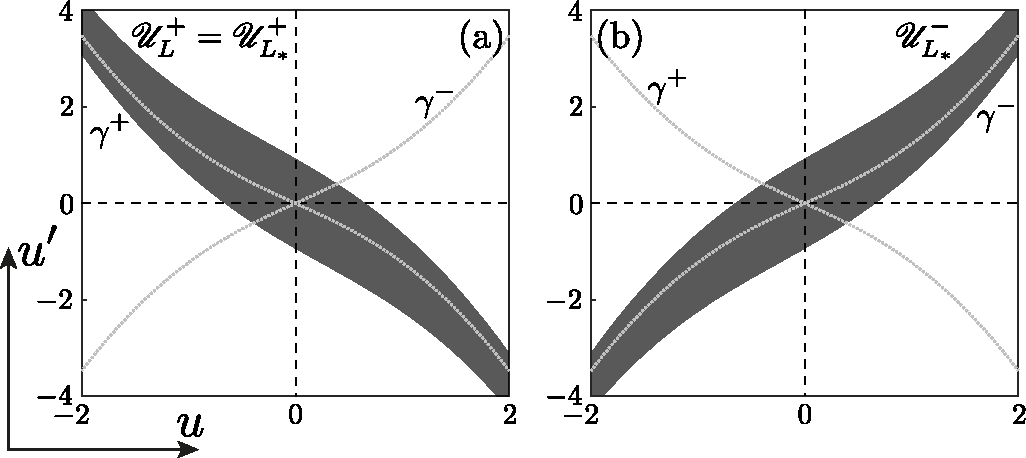
\includegraphics[scale = 1]{pic/Poincare map domain for piecewise singular equation}
	\caption{
		Sets $\mathscr{U}_{L_*}^{\pm}$ for the equation \eqref{eq:stationary-piecewise-singular} for the parameter $L_* = 2$.
		Panel (a) represents $\mathscr{U}_{L_*}^+$ set, it coincides with the set $\mathscr{U}_L^+$ for equation \eqref{eq:stationary-piecewise}, since all solutions of the second equation \eqref{eq:stationary-piecewise-regular} are regular.
		Panel (b) depicts $\mathscr{U}_{L_*}^-$ set, it's just a reflection of the set $\mathscr{U}_L^+$ from the right panel due to Proposition~\ref{prop:domain-reflection}.
	}
\label{fig:poincare-map-domain-piecewise}
\end{figure}

On Figure~\ref{fig:poincare-map-domain-piecewise}~(a) Poincar\'e map   domain $\mathscr{U}_L^+ = \mathscr{U}_{L_*}^+$ for the parameters $(L_*, L_0) = (2, 1)$ is depicted.
As we mentioned above it contains the curve $\gamma^+$ formed by separatrices of \eqref{eq:stationary-piecewise-singular}.
Figure~\ref{fig:poincare-map-domain-piecewise}~(b) represents a $\mathcal{P}_*$-image of $\mathscr{U}_{L_*}^+$, $\mathcal{P}_* (\mathscr{U}_{L_*}^+) = \mathscr{U}_{L_*}^-$.
According to Proposition~\ref{prop:domain-reflection} set $\mathcal{P}_*(\mathscr{U}_{L_*}^-)$ can be obtained by a reflection of the set $\mathscr{U}_{L_*}^+$, with respect to the $u'$ axis.
Set $\mathscr{U}_{L_*}^-$ in its turn contains curve $\gamma^-$.

Let's continue our scanning in order to get set $\mathscr{U}_L^-$ and then intersect it with $\mathscr{U}_L^+$.
On Figure~\ref{fig:island-set-piecewise}~(a) set $\mathscr{U}_L^-$ and its intersection with $\mathscr{U}_L^+$ set are depicted for values of parameters $(L_*, L_0) = (2, 1)$.
From our numerical procedure we can conclude that intersection $\mathscr{U}_L = \mathscr{U}_L^+ \cap \mathscr{U}_L^-$ represents three connected components with monotonic borders.
These components form a three-island set in the scanning area $-2 \le u \le 2$, $-4 \le u' \le 4$, denote them by $D_i, \, i \in \{ -1, 0, +1 \}$.
Indeed, along with the monotonicity of the connected components borders we also know that two opposite borders of $D_i$, which entirely belong to the borders of the set $\mathscr{U}_L^+$, consist of points that are mapped to infinity under action of $\mathcal{P}$ (by construction of $\mathscr{U}_L^+$).
On other hand borders of $\mathscr{U}_L^-$ contain two other borders of each $D_i$, and they are mapped to infinity under action of $\mathcal{P}^{-1}$.
Thereby the obtained structure satisfy all the conditions of island set from Definition~\ref{def:island-set}.
However set $\mathscr{U}_L^-$ entirely contains an image of the curve $\gamma^-$.
We know that according to Proposition~\ref{prop:separatrix-map} image $\mathcal{P}(\gamma^-)$ has infinitely many intersections with the curve $\gamma^+$.
That's why outside of the scanning area there exist many other intersections between sets $\mathscr{U}_L^{\pm}$, and they form infinitely many connected components in the result set $\mathscr{U}_L$.
In a similar manner we denote those components by $D_k$, $k \in \{ -1, -2, -3, \dots \}$ for the components on the left side of the $u'$ axis and $k \in \{ +1, +2, +3, \dots \}$ for the components on the right side. 
Due to monotonicity of $\mathscr{U}_L^+$ borders and general geometric properties of the spiral $\mathscr{U}_L^-$ we can hypothesize that all the components $D_k$ in $\mathscr{U}_L$ set are also islands.

% TODO: Add image of $\gamma^-$ to the pictures.
% TODO: Change color, make it the same as for hypotheses validation figures.
\begin{figure}[h]
\centering
	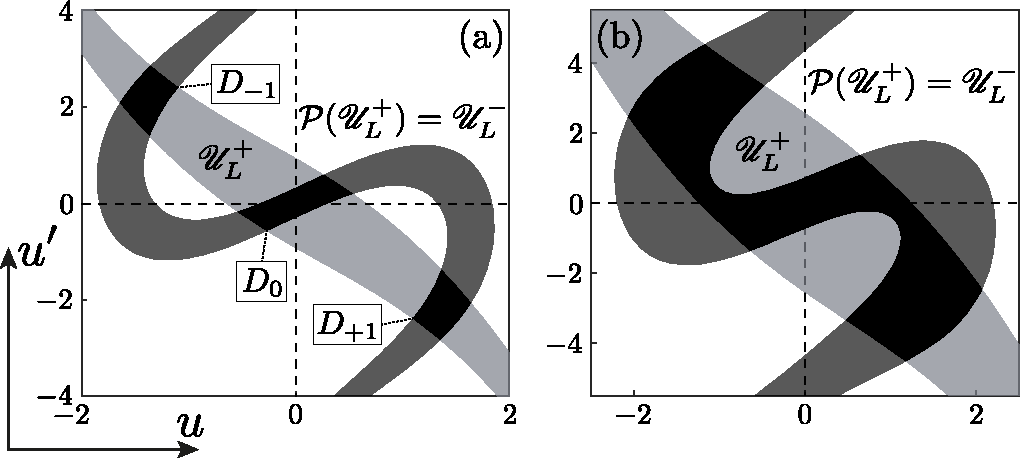
\includegraphics[scale = 1]{pic/island set for piecewise equation}
	\caption{
		Sets $\mathscr{U}_L^+$ (light gray), $\mathscr{U}_L^-$ (dark gray), and their intersection $\mathscr{U}_L$ for two different sets of parameters.
		Panel (a) depict the case $(L_*, L_0) = (2, 1)$; three central connected components $D_i$ form an island set.
		Panel (b) correspond to the case $(L_*, L_0) = (1.3, 1)$; geometry of the result sets does not allow to form islands.
	}
\label{fig:island-set-piecewise}
\end{figure}

Our numerical studies shows that for equation \eqref{eq:stationary-piecewise} three central components of $\mathscr{U}_L$ play a crucial role in an island set formation.
For example in Figure~\ref{fig:islands-set}~(b) geometry of the $\mathscr{U}_L^-$ for parameters $(L_*, L_0) = (1.3, 1)$ does not allow to form an island around the center.
% TODO: Give links to works of Alfimov and Kizin where island set has been studied in details.
Establishing a criteria for existence of the island set is a quite tricky task even for a simple form equation \eqref{eq:stationary-piecewise}, and such criteria is out of scope for the current work.
Our approach is based on scanning of a sufficiently large subset of initial conditions plane around the center $(u, u') = (0, 0)$.
If the resulting subset of $\mathscr{U}_L$ form an island set we just {\it make a hypothesis} that all other intersections and also islands.

\subsection{Complete Island Set}

Let $\mathscr{U}_L$ represents an island set.
It turns out that for Eq.~\eqref{eq:stationary-piecewise} the property of ``completeness''  for an island set in a sense of Definition~\ref{def:complete-island-set} naturally arises from its construction.
Let's demonstrate it in an heuristic manner.
At first, upper boundary of the set $\mathscr{U}_L^+ = \mathscr{U}_{L_*}^+$ consists of such points that the corresponding solution to the Cauchy problem with initial conditions at these points tends to $+\infty$ exactly at the point $x = L_*$.
Therefore, while point $\vb{p}$ is approaching to the upper boundary of $\mathscr{U}_L^+$ it's $\mathcal{P}$-images tends to $(+\infty, +\infty)$.
On other hand lower boundary of $\mathscr{U}_L^+$ consists of points that the corresponding solution to the Cauchy problem with initial conditions at these points tends to $-\infty$.
So, while point $\vb{p}$ is approaching to the lower boundary of $\mathscr{U}_L^+$ it's $\mathcal{P}$-images tends to $(-\infty, -\infty)$.

Let's consider a curve $\Gamma$ inside one of islands $D_i \in \mathscr{U}_L$ that connects opposite boundaries of the set $\mathscr{U}_L^+$.
Denote by $\Gamma_*$ its $\mathcal{P}_*$-image, $\Gamma_* = \mathcal{P}_*(\Gamma)$.
It's clear that $\Gamma_*$ belongs to $\mathscr{U}_{L_*}^-$, and it's stretched out continuously from $-\infty$ to $+\infty$ by $u$ inside $\mathscr{U}_{L_*}^-$.
Now consider the second map $\mathcal{P}_0$ of the decomposition $\mathcal{P} = \mathcal{P}_0 \mathcal{P}_*$.
We know that this map curls the set $\mathscr{U}_{L_*}^-$ into a spiral (see Fig.~\ref{fig:island-set-piecewise}~(a)).
This spiral intersects $\mathscr{U}_L^+$ and form islands.
So if we consider the $\mathcal{P}_0$-image of $\Gamma_*$ and take into account that the value of $H_0$ remains the same for all trajectories of \eqref{eq:stationary-piecewise-regular} associated with $\mathcal{P}_0$ map, we can conclude that $\mathcal{P}_0(\Gamma_*)$ is stretched along the whole set $\mathscr{U}_L^-$ and intersects each of the islands $D_i \in \mathscr{U}_L$ at least once.
Such reasoning leads us to the conclusion that all islands in $\mathscr{U}_L$ are forward-reachable.
Similar consideration shows that islands from $\mathscr{U}_L$ are also backward-reachable and the constructed island set is complete.

Let's illustrate this idea.
For this purpose we construct $\mathcal{P}_*$ and $\mathcal{P}$-images of islands from Figure~\ref{fig:island-set-piecewise}~(a).
Again we do this numerically with the scanning procedure described above.
In Figure~\ref{fig:map-of-islands-piecewise}~(a) one can see the $\mathcal{P}_*$-image of islands $D_i$, $i \in \{ -1, 0, +1\}$.
As we have expected these images are infinite curvilinear strips stretched inside the $\mathcal{P}_*$-image of the $\mathscr{U}_L^+$ set.
$\mathcal{P}$-images of the islands are depicted in Figure~\ref{fig:map-of-islands-piecewise}~(b).
Images $\mathcal{P}(D_i)$ are infinite curvilinear strips curled up inside the $\mathscr{U}_L^-$ set.

\begin{figure}[h]
\centering
	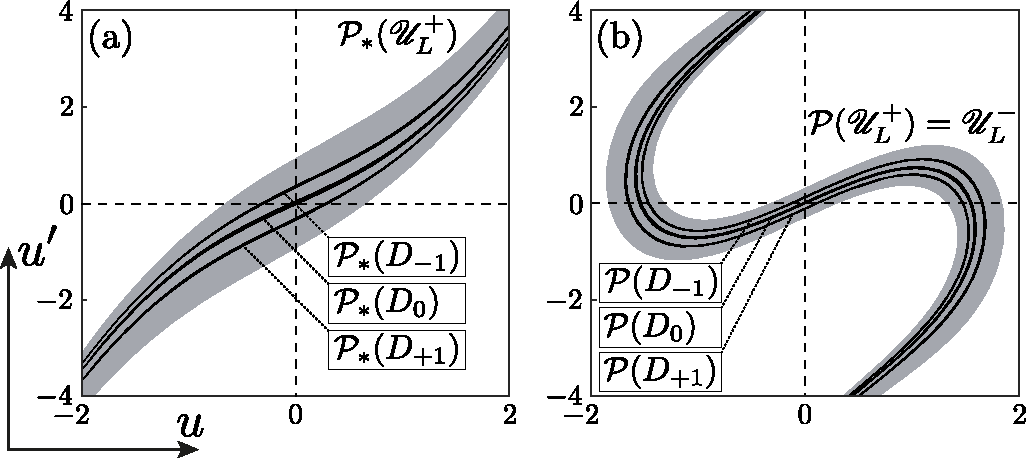
\includegraphics[scale = 1]{pic/Poincare map of islands for piecewise equation}
	\caption{
		$\mathcal{P}_*$ and $\mathcal{P}$-images of islands for Eq.~\eqref{eq:stationary-piecewise} with parameters $(L_*, L_0) = (2, 1)$.
		Panel (a) represents their $\mathcal{P}_*$-images.
		Each image is a curvilinear strip stretched along the whole $\mathcal{P}_*(\mathscr{U}_L^+)$.
		Panel (b) represents $\mathcal{P}$-images.
	}
\label{fig:map-of-islands-piecewise}
\end{figure}

The images $\mathcal{P}(D_i)$ resembles the image $\mathcal{P}_0(\gamma^-)$ of the separatrices $\gamma^-$.
Each of them intersects $\mathscr{U}_L^+$ infinitely many times and cross each island from $\mathscr{U}_L$.
To illustrate this, we combined Figure~\ref{fig:map-of-islands-piecewise}~(b) with Figure~\ref{fig:island-set-piecewise}~(a) in Figure~\ref{fig:h-strips-piecewise} where the notation: $\mathcal{P}(D_i) \cap D_j = H_{ij}$ is introduced.

\begin{figure}[h]
\centering
	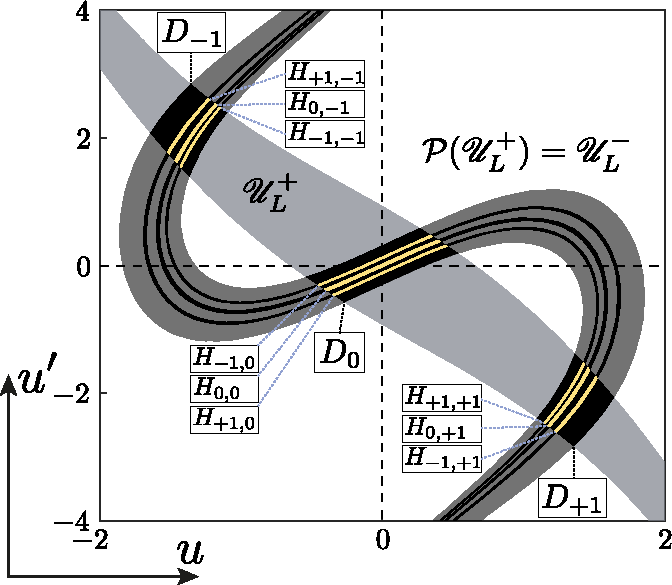
\includegraphics[scale = 1]{pic/h-strips for piecewise equation}
	\caption{
		Island set $\mathscr{U}_L = \mathscr{U}_L^+ \cap \mathscr{U}_L^-$ and sets $H_{ij} = \mathcal{P}(D_i) \cap D_j$, $i, j \in \{ -1, 0, +1 \}$ for equation \eqref{eq:stationary-piecewise} with parameters $(L_*, L_0) = (2, 1)$.
		Island set $\mathscr{U}_L = \bigcup_{i \in S} D_i$ is forward-reachable, so $\mathcal{P}$-image of each island $D_i$ intersects all other islands $D_j$, $j \in S$ including $D_i$ itself.
	}
\label{fig:h-strips-piecewise}
\end{figure}

The similar situation takes place for $\mathcal{P}^{-1}$ map as well.
Island set $\mathscr{U}_L = \bigcup_{i \in S} D_i$ for Eq.~\eqref{eq:stationary-piecewise} is backward-reachable.
It means that $V_{ij} = \mathcal{P}^{-1}(D_j) \cap D_i \neq \varnothing$ for each $i, j \in S$.
In Figure~\ref{fig:v-strips-piecewise} sets $V_{ij}$ are depicted for $i, j \in \{ -1, 0, +1 \}$.

\section{Symbolic Dynamics: Coding of Solutions}

In this section we show how all the concepts introduced above can be used together to classify all bounded solutions of equation \eqref{eq:stationary}.
Our classification is closely connected with the structure of the $\mathscr{U}_L$ set.
We demonstrate our approach for the previously considered piecewise pseudopotential equation \eqref{eq:stationary-piecewise}.
Let's introduce two sets.

\begin{definition}
	Define set $\mathcal{O}$ as a set of bi-infinite orbits of \underline{all} regular solutions for equation \eqref{eq:stationary}, i.e. $\vb{r} \in \mathcal{O}$, $\vb{r} = \{ \vb{p}_n \}$, $\mathcal{P}(\vb{p}_n) = \vb{p}_{n+1}$, $n \in \mathbb{Z}$.
\end{definition}

\begin{figure}[h]
\centering
	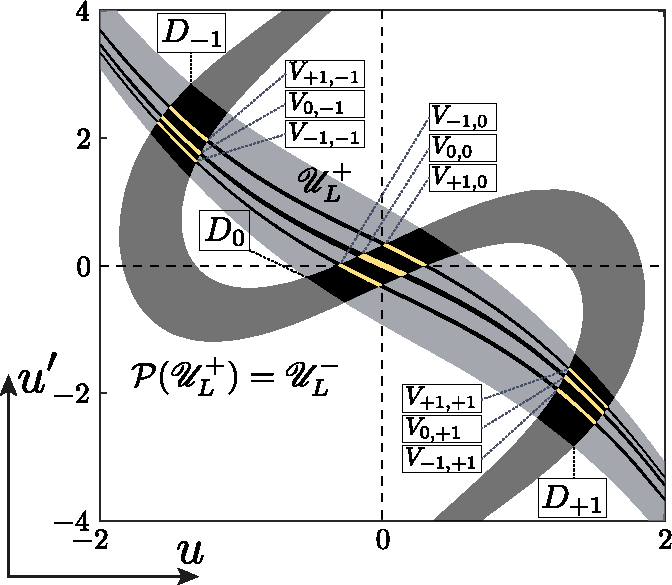
\includegraphics[scale = 1]{pic/v-strips for piecewise equation}
	\caption{
		Island set $\mathscr{U}_L = \mathscr{U}_L^+ \cap \mathscr{U}_L^-$ and sets $V_{ij} = \mathcal{P}^{-1}(D_j) \cap D_i$, $i, j \in \{ -1, 0, +1 \}$ for equation \eqref{eq:stationary-piecewise} with parameters $(L_*, L_0) = (2, 1)$.
		Island set $\mathscr{U}_L = \bigcup_{i \in S} D_i$ is backward-reachable, so $\mathcal{P}$-pre-image of each island $D_i$ intersects all other islands $D_j$, $j \in S$ including $D_i$ itself.
	}
\label{fig:v-strips-piecewise}
\end{figure}

Define a metric in $\mathcal{O}$ as follows.
Let $v, w \in \mathcal{O}$ be two orbits, $v = \{ \vb{p}_n \}$, $\vb{p}_n = (\phi_n, \phi_n')$, $w = \{ \vb{q}_n \}$, $\vb{q}_n = (\psi_n, \psi_n')$, then the distance $d_{\mathcal{O}}$ between orbits $v$ and $w$ is defined as a Euclidean distance between points $\vb{p}_0$ and $\vb{q}_0$, i.e.
\begin{equation}
	d_{\mathcal{O}}(v, w) = ||\vb{p}_0 - \vb{q}_0 || = \sqrt{(\phi_0 - \psi_0)^2 + (\phi_0' - \psi_0')^2}.
\end{equation}
This implies that $\mathcal{O}$ can be regarded as a topological space where neighbourhood $U_{\varepsilon}(u^*)$ of an element $u^* \in \mathcal{O}$ is defined as $U_{\varepsilon}(u^*) = \{u \ | \ d_{\mathcal{O}}(u^*, u) < \varepsilon \}$.

\begin{definition}
	Define set $\mathcal{S}$ as a set of bi-infinite sequences $\{ \dots, i_{-1}, i_0, i_1, \dots \}$ over an alphabet where each symbol $i_k$, $k = 0, \pm 1, \dots$, corresponds to a connected component $D_k \in \mathscr{U}_L$.
\end{definition}

We also write $\mathcal{S}_N$ if the alphabet has $N$ different symbols, and $\mathcal{S}_{\infty}$ if the number of symbols is infinite (corresponds to the infinite number of connected components in $\mathscr{U}_L$).
Set $\mathcal{S}$ also can be regarded as a topological space where neighbourhood $W_k(\omega^*)$ of an element $\omega^* = \{ \dots, i_{-1}^*, i_0^*, i_1^*, \dots \} \in \mathcal{S}$ is defined as $W_k(\omega^*) = \{ \omega \ | \ i_s^* = i_s, |s| < k \}$.

What we are interested in is the connection between sets $\mathcal{O}$ and $\mathcal{S}$.
First of all the structure of island set $\mathscr{U}_L$ can be easily used to assign symbolic sequences, also named codes, to the solutions, so the correspondence from $\mathcal{O}$ to $\mathcal{S}$ can be established.
Let's demonstrate it with an example.
Consider a localized solution $u(x)$ of Eq.~\eqref{eq:stationary-piecewise} shown in the left panel of Figure~\ref{fig:solution-and-orbit}.
Construct the sequence of $(u(kL), u'(kL))$.
On the plane $(u, u')$ each of the points of this sequence is situated in some island $D_i$.
In the point $x = 0$ value $u(0)$ and derivative $u'(0)$ match island $D_{-1}$.
After that in the point $x = L$ our solution $u(x)$ cross the central islands $D_0$ and matches it again for $x = 2L$.
In the point $x = 3L$ our solution came into the right island $D_{+1}$.
That allows us to determine four central symbols of the result code: $\{ -1, 0, 0, +1 \}$, see Figure~\ref{fig:solution-and-orbit}~(b).
Moreover since our solution is localized all other points $(u(kL), u'(kL))$ correspond to the central component of $\mathscr{U}_L$ and all the symbols from the left side of ``$-1$'' and the right side of ``$+1$'' are ``$0$''.
Thereby finally we obtain the result bi-infinite sequence $\{ \dots, 0, -1, 0, 0, +1, 0, \dots \}$ for the localized solution $u(x)$ from Figure~\ref{fig:solution-and-orbit}~(a).
Obviously points of orbit of our solution cannot lie down outside of  $\mathscr{U}_L$ because the solution is regular and has bi-infinite orbit, so at each step we have exactly one symbol to choose and the overall process identifies the result bi-infinite sequence uniquely.

% TODO: place dots exactly where they are on the Panel (b).
\begin{figure}[h]
\centering
	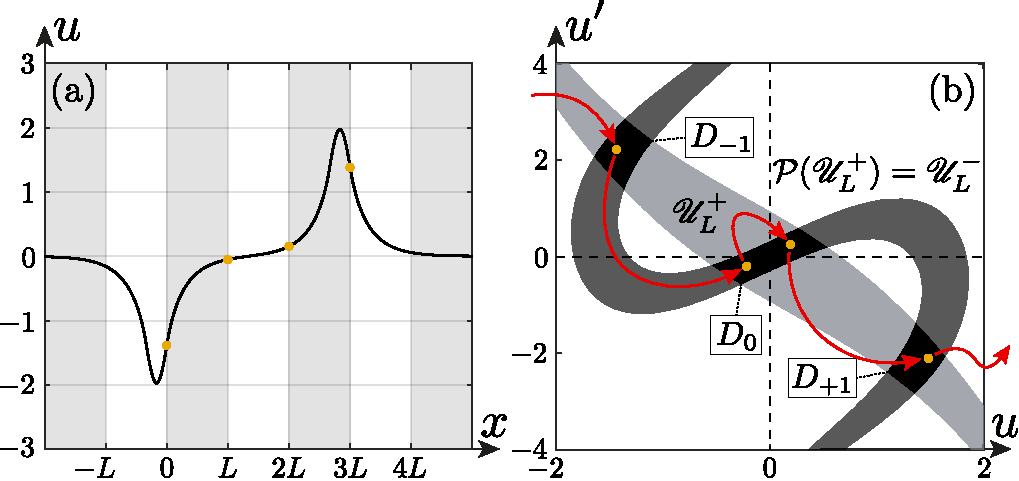
\includegraphics[scale = 1]{pic/solution and orbit on the phase plane}
	\caption{
		Illustration of the coding process.
		Panel~(a) represents a localized solution for the Eq.~\eqref{eq:stationary-piecewise} with parameters $(L_*, L_0) = (2, 1)$.
		This solution has been found numerically using the shooting method.
		Panel~(b) represents a sketch of four points (yellow dots) of the solution orbit over the structure of the $\mathscr{U}_L$ set.
		These points jump from island to island following the red arrows and determine the symbols of the result solution code: $\{ \dots, 0, -1, 0, 0, +1, 0, \dots \}$.
	}
\label{fig:solution-and-orbit}
\end{figure}

\subsection{Uniqueness of Solutions Coding}

The most intriguing question about coding is the following: when is the correspondence between solutions orbits $\mathcal{O}$ and codes $\mathcal{S}$ based on the $\mathscr{U}_L$ set structure for Eq.~\eqref{eq:stationary} is bijective (one-to-one)?
We can also formulate another question: when there exists a homeomorphism between two topological spaces $\mathcal{O}$ and $\mathcal{S}$?
In this section we determine sufficient conditions of existence of such correspondence.

One can reformulate one of the questions above as follows: could one find initial conditions for a Cauchy problem by a solution code?
Let $\vb{s} = \{ \dots, i_{-1}, i_0, i_1, \dots \}$ be a code derived from the structure of a complete island set $\mathscr{U}_L$.
Consider its left part $\{ \dots, i_{-2}, i_{-1}, i_0 \}$.
All the points from island $D_{i_0}$ correspond to the symbol $i_0$.
Consider a set $H_{i_{-1} i_0} = \mathcal{P}(D_{i_{-1}}) \cap D_{i_0}$.
The set $H_{i_{-1} i_0} \subset D_{i_0}$ consists of such points $\vb{p}_0 = (u_0, u_0') \in D_{i_0}$ that the corresponding solution $u(x)$ to the Cauchy problem with initial conditions $u(0) = u_0$, $u'(0) = u_0'$ does not collapse at $[-L; 0]$, and $\vb{p}_{-1} = (u(-L), u'(-L)) \in D_{i_{-1}}$.
Hence the code of solution with initial conditions taken from $H_{i_{-1}, i_0}$ includes symbols $\{ i_{-1}, i_0 \}$.
Continuing this process.
Consider a set $H_{i_{-2}, i_{-1}, i_0} = \mathcal{P}(H_{i_{-2}, i_{-1}}) \cap D_{i_0}$, where $H_{i_{-2}, i_{-1}} = \mathcal{P}(D_{i_{-2}}) \cap D_{i_{-1}}$.
The set $H_{i_{-2}, i_{-1}, i_0} \subset D_{i_0}$ consists of such points $\vb{p}_0 = (u_0, u_0') \in D_{i_0}$ that the corresponding solution $u(x)$ to the Cauchy problem with initial conditions $u(0) = u_0$, $u'(0) = u_0'$ does not collapse at $[-2L; 0]$, and $\vb{p}_{-1} = (u(-L), u'(-L)) \in D_{i_{-1}}$, $\vb{p}_{-2} = (u(-2L), u'(-2L)) \in D_{i_{-2}}$.
That's why the code of solution with initial conditions taken from $H_{i_{-2}, i_{-1}, i_0}$ includes symbols $\{ i_{-2}, i_{-1}, i_0 \}$.

In order to formalize this process we introduce an arrow operator $X \xrightarrow{\mathcal{P}} Y = \mathcal{P}(X) \cap Y$.
This operator is not associative and should be applied strictly from left to right, i.e. $X \xrightarrow{\mathcal{P}} Y \xrightarrow{\mathcal{P}} Z = (\mathcal{P}(X) \cap Y) \xrightarrow{\mathcal{P}} Z$.
Consider a sequence of nested sets:
\begin{equation}
	\begin{alignedat}{2}
		& D_{i_0} \supseteq H_{i_0} && \ = D_{i_0}; \\
		& D_{i_0} \supseteq H_{i_{-1}, i_0} && \ = D_{i_{-1}} \xrightarrow{\mathcal{P}} D_{i_0}; \\
		& D_{i_0} \supseteq H_{i_{-2}, i_{-1}, i_0} && \ = D_{i_{-2}} \xrightarrow{\mathcal{P}} D_{i_{-1}} \xrightarrow{\mathcal{P}} D_{i_0}; \\
		& D_{i_0} \supseteq H_{i_{-3}, i_{-2}, i_{-1}, i_0} && \ = D_{i_{-3}} \xrightarrow{\mathcal{P}} D_{i_{-2}} \xrightarrow{\mathcal{P}} D_{i_{-1}} \xrightarrow{\mathcal{P}} D_{i_0}; \\
		& \dots.
	\end{alignedat}
\label{eq:nested-h-sets}
\end{equation}
All of them are situated inside the island $D_{i_0}$, moreover all of sets $H_{i_{-k}, \dots, i_0}$ are non-empty due to completeness of the island set $\mathscr{U}_L$.
Consider an intersection of these sets $H_{\infty} = \bigcap_{k = 0}^{\infty} H_{i_{-k}, \dots, i_0}$.
By the construction resulting set $H_{\infty}$, if non-empty, consists of such points that the corresponding solution with initial conditions $u(0) = u_0$, $u'(0) = u_0'$, $(u_0, u_0') \in H_{\infty}$, exists on the interval $(-\infty; 0]$ and its code coincide with the left part of the initially considered sequence $\vb{s}$.

Let's do the similar operations with the right part of $\vb{s}$: $\{ i_0, i_1, i_2, \dots \}$.
Consider a sequence of nested sets:
\begin{alignat*}{2}
	& D_{i_0} \supseteq V_{i_0} && \ = D_{i_0}; \\
	& D_{i_0} \supseteq V_{i_0, i_1} && \ = D_{i_1} \xrightarrow{\mathcal{P}^{-1}} D_{i_0}; \\
	& D_{i_0} \supseteq V_{i_0, i_1, i_2} && \ = D_{i_2} \xrightarrow{\mathcal{P}^{-1}} D_{i_1} \xrightarrow{\mathcal{P}^{-1}} D_{i_0}; \\
	& D_{i_0} \supseteq V_{i_0, i_1, i_2, i_3} && \ = D_{i_3} \xrightarrow{\mathcal{P}^{-1}} D_{i_2} \xrightarrow{\mathcal{P}^{-1}} D_{i_1} \xrightarrow{\mathcal{P}^{-1}} D_{i_0}; \\
	& \dots.
\end{alignat*}
All of these nested sets $V_{i_0, \dots, i_k}$ are situated inside the island $D_{i_0}$ and are non-empty.
Consider an intersections $V_{\infty} = \bigcap_{k = 0}^{\infty} V_{i_0, \dots, i_k}$.
Set $V_{\infty}$, if non-empty, consists of such points that solution with initial conditions from $V_{\infty}$ exists on the interval $[0; +\infty)$ and its code coincide with the right part of $\vb{s}$.

Intersection of these two sets $H_{\infty} \cap V_{\infty}$ consists of such points of initial conditions that gives the result regular solutions with the desired code $\vb{s}$.
The geometry of $H_{\infty} \cap V_{\infty}$ can be quite complex.
But if the intersection consists of just one point then we can say that the code identifies a solution uniquely.

Our goal is to formulate sufficient conditions that allows us to state that any bi-infinite code identify a regular solution uniquely.
Again let $\mathscr{U}_L$ represent a complete island set for equation of type \eqref{eq:stationary}.
Consider the sequences of nested sets:
\begin{alignat*}{6}
	& \mathscr{U}_L = \mathscr{H}_0 && \supseteq \mathscr{H}_1 && \supseteq \mathscr{H}_2 && \supseteq \mathscr{H}_3 && \supseteq \dots, \quad && \mathscr{H}_i = \mathcal{P}(\mathscr{H}_{i-1}) \cap \mathscr{H}_0; \\
	& \mathscr{U}_L = \mathscr{V}_0 && \supseteq \mathscr{V}_1 && \supseteq \mathscr{V}_2 && \supseteq \mathscr{V}_3 && \supseteq \dots, \quad && \mathscr{V}_i = \mathcal{P}^{-1}(\mathscr{V}_{i-1}) \cap \mathscr{V}_0.
\end{alignat*} 
Define the following sets as intersections of the sequences above:
\begin{alignat*}{6}
	& \mathscr{H}_{\infty} && = \mathscr{H}_0 && \cap \mathscr{H}_1 && \cap \mathscr{H}_2 && \cap \mathscr{H}_3 && \cap \dots; \\
	& \mathscr{V}_{\infty} && = \mathscr{V}_0 && \cap \mathscr{V}_1 && \cap \mathscr{V}_2 && \cap \mathscr{V}_3 && \cap \dots.
\end{alignat*}
By its construction their intersection $\mathscr{U}_{\infty} = \mathscr{H}_{\infty} \cap \mathscr{V}_{\infty}$ contains initial conditions for all regular solutions of equation \eqref{eq:stationary}.
Set $\mathscr{U}_{\infty}$ is a central object for describing of the set of regular solutions for equation of such type \cite{AlfimovAvramenko, AlfimovLebedev, AlfimovKizinZezyulin}.
Its structure may be quite sophisticated having a form of a complex fractal set.
One can have a nice illustration on how this set may look like for equation \eqref{eq:stationary-piecewise}.
For that purpose we combine Figure~\ref{fig:h-strips-piecewise} and Figure~\ref{fig:v-strips-piecewise} into a single plot.

\begin{figure}[h]
\centering
	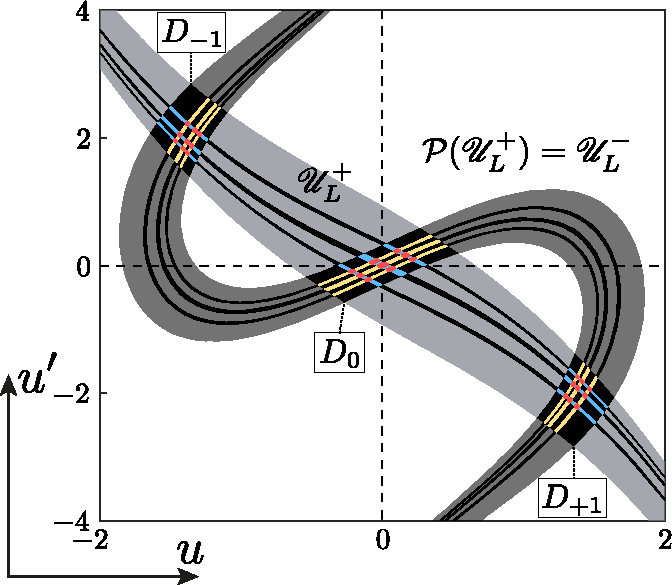
\includegraphics[scale = 1]{pic/h- and v-strips for piecewise equation}
	\caption{
		Subsets of $\mathscr{H}_1$ (yellow) and $\mathscr{V}_1$ (blue), and their intersection $\mathscr{H}_1 \cap \mathscr{V}_1$ (magenta).
		This figure give an illustration on how the partitioning inside the set $\mathscr{U}_L$ (black) starts to occur while considering higher orders of $\mathcal{P}$ and $\mathcal{P}^{-1}$.
	}
\label{fig:hv-strips-piecewise}
\end{figure}

In Figure~\ref{fig:hv-strips-piecewise} subsets of $\mathscr{H}_1$ (yellow) and $\mathscr{V}_1$ (blue) along with their intersection $\mathscr{H}_1 \cap \mathscr{V}_1$ (magenta) are presented.
There exist other parts of $\mathscr{H}_1$ and $\mathscr{V}_1$ that can be obtained by considering $\mathcal{P}$ and $\mathcal{P}^{-1}$-images of other islands lying outside of the scanning area, but we exclude them for the sake of clarity.
One can see how the partitioning inside the $\mathscr{U}_L$ occurs.
Continuation of that process with higher orders of maps $\mathcal{P}$ and $\mathcal{P}^{-1}$ results in additional partitioning inside the set $\mathscr{H}_1 \cap \mathscr{V}_1$ and reveals the complex nature of the set $\mathscr{U}_{\infty}$.
Eventually if for each code there exists exactly one point of initial conditions in the set $\mathscr{U}_{\infty}$ then we can state the existence of one-to-one correspondence between regular solutions and symbolic sequences derived from the structure of the set $\mathscr{U}_L$.
Let's now formulate the sufficient conditions of that.
We do this in a form of two hypotheses which are of the form of so-called Conley--Moser conditions \cite[Chapter 25]{Wiggins}.

% TODO: make a remark on infinite indices set $S$.
\begin{hypothesis}
\label{hypothesis:island-set}
	For equation \eqref{eq:stationary} with $L$-periodic functions $Q(x)$, $P(x)$ the set $\mathscr{U}_L$ is a complete island set, $\mathscr{U}_L = \bigcup_{i \in S} D_i$, and there exist constants $M, N$ such that $d_{\emph{h}}(D_i) \le M$ and $d_{\emph{v}}(D_i) \le N$ for any $i \in S$.
\end{hypothesis}

\begin{hypothesis}
\label{hypothesis:strips-mapping}
	Let $\mathscr{U}_L = \bigcup_{i \in S} D_i$ be an island set.
	For each $i, j \in S$ there exist $\gamma_{ij}$ such that for any \emph{h}-strip $H \in D_i$ its $\mathcal{P}$-image $\widetilde{H}_j = \mathcal{P}(H) \cap D_j$ is an $\mathrm{h}_{\gamma_{ij}}$-strip, and there exists $\mu > 1$ such that
	\begin{equation}
		d_{\mathrm{h}}(\widetilde{H}_j) \le (1/\mu) d_{\mathrm{h}}(H).
	\end{equation}
	For each $i, j \in S$ there exist $\delta_{ij}$ such that for and any \emph{v}-strip $V \in D_j$ its $\mathcal{P}$-pre-image $\widetilde{V}_i = \mathcal{P}^{-1}(V) \cap D_i$ is a $\mathrm{v}_{\delta_{ij}}$-strip, and there exists $\nu > 1$ such that
	\begin{equation}
		d_{\mathrm{v}}(\widetilde{V}_i) \le (1/\nu) d_{\mathrm{v}}(V).
	\end{equation}
\end{hypothesis}

Two hypotheses introduced above allow us to formulate and prove the central theorem (Theorem~\ref{thm:coding}) of our coding approach.
This theorem partially reproduce the result initially proved in \cite[Theorem 3.1]{AlfimovAvramenko}.
However Theorem~\ref{thm:coding} turns out to be more suitable for further numerical analysis, since we excluded Hypothesis~III from \cite{AlfimovAvramenko} and replaced it with modified version of Hypothesis~\ref{hypothesis:strips-mapping}.
Hypothesis~III from \cite{AlfimovAvramenko} requires a sophisticated analyses of areas of sets $D_i$ in plane which is hard to perform numerically.

% TODO: Consider to name this theorem somehow.
\begin{theorem}
	Assume that Poincar\'e map associated with equation \eqref{eq:stationary} satisfies Hypotheses \ref{hypothesis:island-set} and \ref{hypothesis:strips-mapping}.
	Then there exists a homeomorphism of topological spaces\footnote{We use the symbol $\mathcal{C}$ for the homeomorphism since it reminds the overall process as ``coding''.} $\mathcal{C}: \mathcal{O} \to \mathcal{S}$, defined as follows: $\mathcal{C}(\vb{r}) = \vb{s}$, $\vb{r} \in \mathcal{O}$, $\vb{r} = \{ \vb{p}_k \}$ and $\vb{s} \in \mathcal{S}$, $\vb{s} = \{ i_k \}$, such that $i_k$ is the number of the component $D_{i_k} \in \mathscr{U}_L$ where the point $\vb{p}_k$ lies.
\label{thm:coding}
\end{theorem}
\begin{proof}
	Evidently, for each bi-infinite orbit $\vb{r} \in \mathcal{O}$ of regular solution the image $\vb{s} = \mathcal{C}(\vb{r})$, $\vb{s} \in \mathcal{S}$ is defined uniquely.
	Let's prove that for each sequence $\vb{s} \in \mathcal{S}$ there exist unique orbit $\vb{r} \in \mathcal{O}$ such that $\vb{s} = \mathcal{C}(\vb{r})$.
	
	Consider a sequence $\vb{s} = \{ \dots, i_{-1}, i_0, i_1, \dots \}$.
	Let's find a location of the points $\vb{p} \in D_{i_0}$ such that $\mathcal{P}^{-1}(\vb{p}) \in D_{i_{-1}}$, $\mathcal{P}^{-2}(\vb{p}) \in D_{i_{-2}}$, etc.
	First of all, $D_{i_0}$ is a $\gamma_{i_0}$-island, then it's an $\mathrm{h}_{\gamma_{i_0}}$-strip.
	Define an $\mathrm{h}_{\gamma_{i_0}}$-strip $H_{i_0} = D_{i_0}$ as a base step.
	From Hypothesis~\ref{hypothesis:island-set} we conclude that
		\begin{equation}
		d_{\mathrm{h}}(H_{i_0}) \le M.
	\end{equation}
	Points $\vb{p} \in D_{i_0}$ such that $\mathcal{P}^{-1}(\vb{p}) \in D_{i_{-1}}$ are situated in the set $H_{i_{-1}, i_0} = \mathcal{P}(D_{i_{-1}}) \cap D_{i_0}$.
	Due to Hypothesis~\ref{hypothesis:strips-mapping} set $H_{i_{-1}, i_0}$ is an $\mathrm{h}_{\gamma_{i_0, i_{-1}}}$-strip.
	Its thickness satisfies an inequality
	\begin{equation}
		d_{\mathrm{h}}(H_{i_{-1}, i_0}) \le \mu^{-1} d_{\mathrm{h}}(H_{i_0}) \le \mu^{-1} M.
	\end{equation}
	For simplicity define $\gamma = \max \{ \gamma_{i_0}, \gamma_{i_0, i_{-1}} \}$.
	
	Points $\vb{p} \in D_{i_0}$ such that $\mathcal{P}^{-1}(\vb{p}) \in D_{i_{-1}}$, $\mathcal{P}^{-2}(\vb{p}) \in D_{i_{-2}}$ are situated in the set $H_{i_{-2}, i_{-1}, i_0} = \mathcal{P}(H_{i_{-2}, i_{-1}}) \cap D_{i_0}$ where $H_{i_{-2}, i_{-1}} = \mathcal{P}(D_{i_{-2}}) \cap D_{i_{-1}}$.
	By Hypothesis~\ref{hypothesis:strips-mapping} set $H_{i_{-2}, i_{-1}}$ is an h-strip.
	Hence, set $H_{i_{-2}, i_{-1}, i_0}$ is an $\mathrm{h}_{\gamma}$-strip and its thickness satisfies an inequality
	\begin{equation}
		d_{\mathrm{h}}(H_{i_{-2}, i_{-1}, i_0}) \le \mu^{-1} d_{\mathrm{h}}(H_{i_{-2}, i_{-1}}) \le \mu^{-2} d_{\mathrm{h}}(D_{i_{-2}}) \le \mu^{-2} M.
	\end{equation}
	
	Continuation of that process leads us to the sequence of nested $\mathrm{h}_{\gamma}$-strips similar to what we had in \eqref{eq:nested-h-sets}:
	\begin{equation}
		D_{i_0} = H_{i_0} \supseteq H_{i_{-1}, i_0} \supseteq H_{i_{-2}, i_{-1}, i_0} \supseteq \dots.
	\label{eq:nested-h-strips}
	\end{equation}
	Let's show that the infinite intersection of the $\mathrm{h}_{\gamma}$-strips \eqref{eq:nested-h-strips} is an $\mathrm{h}_{\gamma}$-curve.
	Sequence of their thicknesses is bounded from above with a decreasing sequence $\{ \mu^{-n} M \}$, $n = 0, 1, 2, \dots$.
	Value $\mu > 1$, so the limit $\lim \limits_{n \to \infty} \mu^{-n} M = 0$.	
	Now consider boundaries of the strips \eqref{eq:nested-h-sets} as a functions of $u$.
	All of them are $\gamma$-Lipschitz functions.
	Their domains are different, but all of them lie inside the domain $\Delta$, defined as
	\begin{equation}
		\Delta = \mathrm{dom}(\alpha_{i_0}^+) \cup \mathrm{dom}(\alpha_{i_0}^-),
	\end{equation}
	where $\alpha_{i_0}^{\pm}$ are opposite boundaries of the first strip $H_{i_0}$.
	We can continue each $\alpha^{\pm}$ boundary of h-strips \eqref{eq:nested-h-sets} onto the whole $\Delta$.
	Let $\alpha_{i_{-k}, \dots, i_0}^{\pm}$ be a boundaries of an h-strip $H_{i_{-k}, \dots, i_0}$.
	They can be considered as a functions of $u$, $u' = h_{i_{-k}, \dots, i_0}^{\pm}(u)$ with the domains $\Delta_{i_{-k}, \dots, i_0}^{\pm} = [a_{i_{-k}, \dots, i_0}^{\pm}; b_{i_{-k}, \dots, i_0}^{\pm}]$, and we can define new functions
	\begin{equation}
		\widetilde{h}_{i_{-k}, \dots, i_0}^{\pm}(u) = \begin{cases}
			h_{i_{-k}, \dots, i_0}^{\pm}(a_{i_{-k}, \dots, i_0}^{\pm}) & u < a_{i_{-k}, \dots, i_0}^{\pm}; \\
			h_{i_{-k}, \dots, i_0}^{\pm}(u) & u \in \Delta_{i_{-k}, \dots, i_0}^{\pm}; \\
			h_{i_{-k}, \dots, i_0}^{\pm}(b_{i_{-k}, \dots, i_0}^{\pm}) & u > b_{i_{-k}, \dots, i_0}^{\pm}.
		\end{cases}
	\label{eq:nested-h-strips-extension}
	\end{equation}
	Such extension allows us to treat boundaries of $H_{{i_{-k}, \dots, i_0}}$ as functions of $u$ with the same domain and consider them as a part of the space $C_{\gamma}(\Delta)$ of $\gamma$-Lipschitz functions defined on the interval $\Delta$.
	Definition of the h-strip thickness coincide with the metric defined by the maximum norm, and $C_{\gamma}(\Delta)$ is a complete metric space \cite{Arnold}.
	Now consider the sequence
	\begin{equation}
		\{ \widetilde{h}_{i_0}^+(u), \widetilde{h}_{i_0}^-(u), \widetilde{h}_{i_{-1}, i_0}^+, \widetilde{h}_{i_{-1}, i_0}^-, \dots, \widetilde{h}_{i_{-k}, \dots, i_0}^+, \widetilde{h}_{i_{-k}, \dots, i_0}^-, \dots \}.
	\label{eq:sequence-of-boundaries}
	\end{equation}
	Since $H_{i_{-k}, \dots, i_0} \subseteq H_{i_{-k+1, \dots i_0}}$ and $d_{\mathrm{h}}(H_{i_{-k}, \dots, i_0}) \to 0$ as $k \to \infty$, sequence \eqref{eq:sequence-of-boundaries} is a Cauchy sequence.
	Therefore, since $C_{\gamma}(\Delta)$ is a complete metric space, the Cauchy sequence converges to a unique curve $\widetilde{h}_{\infty}(u)$ which represents an $\mathrm{h}_{\gamma}$-curve inside the island $D_{i_0}$.
	Since we extend h-strips boundaries onto the whole $\Delta$ there may be other parts of $\widetilde{h}_{\infty}(u)$ lying outside of $D_{i_0}$.
	Denote by $\alpha_{\infty}$ a part of $\widetilde{h}_{\infty}(u)$ that entirely belongs to $D_{i_0}$.
	This curve is the intersection of the $\mathrm{h}_{\gamma}$-strips \eqref{eq:nested-h-strips} and is an $\mathrm{h}_{\gamma}$-curve.
	
	In the same manner a sequence of nested $\mathrm{v}_{\delta}$-strips can be constructed,
	\begin{equation}
		D_{i_0} = V_{i_0} \supseteq V_{i_0, i_1} \supseteq V_{i_0, i_1, i_2} \supseteq \dots.
	\label{eq:nested-v-strips}
	\end{equation}
	Their thicknesses are bounded from above with a decreasing sequence $\{ \nu^{-n} N \}$, $n = 0, 1, 2, \dots$ of a zero limit, $\lim \limits_{n \to \infty} \nu^{-n} N = 0$.
	Considering a corresponding sequence of $\delta$-Lipschitz functions we conclude that the intersection of the strips \eqref{eq:nested-v-strips} exists and is a $\mathrm{v}_\delta$-curve.
	Denote this curve by $\beta_{\infty}$.
	
	The orbit $\vb{r} \in \mathcal{O}$ corresponding to the bi-infinite sequence $\{ \dots, i_{-1}, i_0, i_1, \dots \}$ is generated by $\mathcal{P}$ and $\mathcal{P}^{-1}$-iterations of the intersection $\alpha_{\infty} \cap \beta_{\infty}$ which according to the definitions of h- and v-curves {\it consists of one point}.
	Therefore orbit $\vb{r}$ exists and is unique.
	
	The continuity of $\mathcal{C}$ and $\mathcal{C}^{-1}$ maps follows from an observation that follows below.
	Since $\mathcal{P}$ is continuous, if $\vb{r}^{(1)}, \vb{r}^{(2)} \in \mathcal{O}$,
	\begin{eqnarray*}
		& \vb{r}^{(1)} = \{ \dots, \vb{p}_{-1}^{(1)}, \vb{p}_0^{(1)}, \vb{p}_1^{(1)}, \dots \}, \\
		& \vb{r}^{(2)} = \{ \dots, \vb{p}_{-1}^{(2)}, \vb{p}_0^{(2)}, \vb{p}_1^{(2)}, \dots \};
	\end{eqnarray*}
	are close enough in $\mathcal{O}$ (i.e. points $\vb{p}_0^{(1)}$ and $\vb{p}_0^{(2)}$ are close in $\mathbb{R}^2$), then their $\mathcal{C}$-images share the same central block $|k| < n$ for some $n$.
	Therefore they are also close in $\mathcal{S}$-topology.
	If $\vb{s}^{(1)} = \mathcal{C}(\vb{p}^{(1)})$ and $\vb{s}^{(2)} = \mathcal{C}(\vb{p}^{(2)})$ share the same central block $|k| < n$ for some $n$ then the points $\vb{p}_0^{(1)}$ and $\vb{p}_0^{(2)}$ are situated in the same area $H_{i_{-k}, \dots, i_0} \cap V_{i_0, \dots, i_k}$, so $\vb{p}_0^{(1)}$ and $\vb{p}_0^{(2)}$ are close in $\mathcal{O}$-topology.
	Theorem is proven.
\end{proof}

\section{Numerical Test of Existence of Coding Homeomorphism}

In order to apply Theorem~\ref{thm:coding} to equation \eqref{eq:stationary} one should get a strong evidence that Hypotheses \ref{hypothesis:island-set} and \ref{hypothesis:strips-mapping} are valid.
However it's rather difficult to obtain a rigorous mathematical proof of them even for the simplest form of the functions $Q(x)$, $P(x)$ in \eqref{eq:stationary}.
Instead, in our current work we provide a computing procedure that allows to check numerically that Hypotheses~\ref{hypothesis:island-set} and \ref{hypothesis:strips-mapping} are valid at least at finite domain of plane of initial conditions.
Hypothesis~\ref{hypothesis:island-set} can be verified in a straightforward way, since we can apply the scanning procedure and get a structure of the set $\mathscr{U}_L$.
There may be two possible scenarios.

The \underline{first} scenario is when we can prove that the set $\mathscr{U}_L$ is bounded within a finite domain, like the authors of the work \cite{AlfimovAvramenko} did for $P(x) \equiv -1$.
Then one can apply a scanning procedure to that domain and thus provide a numerical evidence that Hypothesis~\ref{hypothesis:island-set} holds for the whole set $\mathscr{U}_L$.

The \underline{second} scenario is when we cannot prove any statement on the boundaries and structure of $\mathscr{U}_L$, or this set is infinite and unbounded.
For example, we saw previously that for equation \eqref{eq:stationary-piecewise} set $\mathscr{U}_L$ is unbounded.
In that case we cannot compute the whole set $\mathscr{U}_L$, since it's possible to scan only a finite subset of the initial conditions plane.
But if the finite subset of $\mathscr{U}_L$ represents an island set of $N$ islands, the coding approach still can be possibly applied.
Let's denote $\mathcal{D}_N = \bigcup_{k \in S_N} D_k$ the finite subset of $N$ islands from $\mathscr{U}_L$, obtained by the scanning procedure.
We can reduce our consideration to regular solutions which orbits visit only islands from $\mathcal{D}_N$.
Let $\mathcal{O}_N \subset \mathcal{O}$ denote a subset of such orbits.
If Hypothesis~\ref{hypothesis:strips-mapping} is valid for the $\mathcal{D}_N$, we can conclude that conditions of Theorem~\ref{thm:coding} are met and there exists a homeomorphism between a {\it subset of orbits of regular solutions} $\mathcal{O}_N$ and set of bi-infinite sequences $\mathcal{S}_N$ of symbols from finite set $S_N$.

Hypothesis~\ref{hypothesis:strips-mapping} does not admit straightforward numerical verification by itself.
However, it can be reduced to another two statements, called Strips Mapping Theorems, which admit numerical verification.
This statements rely on properties of linear operators $D \mathcal{P}_{\vb{p}}$, $D \mathcal{P}^{-1}_{\vb{p}}$, which are represented by the Jacobi matrices of $\mathcal{P}$ and $\mathcal{P}^{-1}$, 
\begin{alignat}{4}
	& \mathcal{P}(\vb{q}) && = \mathcal{P}(\vb{p}) && + D \mathcal{P}_{\vb{p}} (\vb{q} - \vb{p}) && + o(||\vb{q} - \vb{p}||); \\
	& \mathcal{P}^{-1}(\vb{q}) && = \mathcal{P}^{-1}(\vb{p}) && + D \mathcal{P}^{-1}_{\vb{p}} (\vb{q} - \vb{p}) && + o(||\vb{q} - \vb{p}||).
\end{alignat}
Let's formulate the first statement that cover a part of Hypothesis~\ref{hypothesis:island-set} related to the h-strips mapping.

\begin{theorem}[On h-strips mapping]
\label{thm:h-strips-mapping}
	Let Poincar\'e map $\mathcal{P}$ and its inverse $\mathcal{P}^{-1}$ be defined on a complete (see Definition~\ref{def:complete-island-set}) island set $\bigcup_{i \in S} D_i$, where $S$ is a finite or countable set of indices.
	Let for all $i, j \in S$ the set $V_{ij} = \mathcal{P}^{-1} (D_j) \cap D_i$ is non-empty, $\mathcal{P}$ is defined on a closure $\overline{V_{ij}}$, and one of the following two conditions holds:
	\begin{enumerate}
		\item[(1)] the borders $\alpha_i^{\pm}$ of an island $D_i$ are increasing curves, $\forall \vb{p} \in \overline{V_{ij}}$ the signs of $\{ a_{mn} \}$ in the matrix of the linear operator $D \mathcal{P}_{\vb{p}} = (a_{mn})$ have exactly one of the following configurations\footnote{By ``$+$'' and ``$-$'' sign we mean \underline{strict} inequalities $a_{mn} > 0$, $a_{mn} < 0$ to be held.}:
			\begin{center}
				(a) $\begin{psm} + & + \\ + & + \end{psm}$, \quad
				(b) $\begin{psm} - & - \\ - & - \end{psm}$, \quad
				(c) $\begin{psm} + & + \\ - & - \end{psm}$, \quad
				(d) $\begin{psm} - & - \\ + & + \end{psm}$;
			\end{center}
			and at the same time the borders $\alpha_j^{\pm}$ of $D_j$ are increasing curves for cases (a), (b), and decreasing curves for (c), (d);
		\item[(2)] the borders $\alpha_i^{\pm}$ of an island $D_i$ are decreasing curves, $\forall \vb{p} \in \overline{V_{ij}}$ signs of $\{ a_{mn} \}$ in the matrix of the linear operator $D \mathcal{P}_{\vb{p}} = (a_{mn})$ have exactly one of the following configurations:
			\begin{center}
				(a) $\begin{psm} + & - \\ - & + \end{psm}$, \quad
				(b) $\begin{psm} - & + \\ + & - \end{psm}$,	\quad
				(c) $\begin{psm} + & - \\ + & - \end{psm}$, \quad
				(d) $\begin{psm} - & + \\ - & + \end{psm}$;		
			\end{center}
			and at the same time borders $\alpha_j^{\pm}$ of $D_j$ are decreasing curves for cases (a), (b), and increasing for (c), (d);
	\end{enumerate}
	and moreover $\exists \mu > 1$ such that $\forall p \in \overline{V_{ij}}$, $|a_{11}| \ge \mu$.
	Then
	\begin{itemize}
		\item[(i)] for any \emph{h}-strip $H \in D_i$, $\mathcal{P} (H) \cap D_j = \widetilde{H}_j$ is also an \emph{h}-strip;
		\item[(ii)] $d_{\mathrm{h}}(\widetilde{H}_j) \le (1 / \mu) d_{\mathrm{h}}(H)$ (here $d_{\mathrm{h}}(\cdot)$ is an \emph{h}-strip thickness in a sence of Definition~\ref{def:h-thickness}).
	\end{itemize}
\end{theorem}
Proof of Theorem~\ref{thm:h-strips-mapping} can be found in Appendix~\ref{appendix:strips-mapping-theorems}.
Basically, this theorem postulate two following things:
\begin{itemize}
	\item If linear operator $D \mathcal{P}_{\vb{p}} = (a_{mn})$, $\vb{p} \in V_{ij}$, satisfies {\it some conditions} about signs of $a_{mn}$, then $\mathcal{P}$ {\it maps h-strips to h-strips}.
	\item If for the linear operator $D \mathcal{P}_{\vb{p}} = (a_{mn})$ the estimation $|a_{11}| \ge \mu > 1$, takes place for $\vb{p} \in V_{ij}$ ($\exists \mu$), then $\mathcal{P}$ {\it shrinks thickness of h-strips}.
\end{itemize}
The next theorem establish the similar properties for the v-strips mapping.

\begin{theorem}[On v-strips mapping]
\label{thm:v-strips-mapping}
	Let Poincar\'e map $\mathcal{P}$ and its inverse $\mathcal{P}^{-1}$ be defined on a complete (see Definition~\ref{def:complete-island-set}) island set $\bigcup_{i \in S} D_i$, where $S$ is a finite or countable set of indices.
	Let for all $i, j \in S$ the set $H_{ij} = \mathcal{P} (D_i) \cap D_j$ is non-empty, $\mathcal{P}^{-1}$ is defined on a
	 closure $\overline{H_{ij}}$, and one of the following two conditions holds:
	\begin{enumerate}
		\item[(1)] the borders $\beta_j^{\pm}$ of an island $D_j$ are increasing curves, $\forall \vb{q} \in \overline{H_{ij}}$ the signs of $\{ b_{mn} \}$ in the matrix of the linear operator $D \mathcal{P}_{\vb{q}}^{-1} = (b_{mn})$ have exactly one of the following configurations:
			\begin{center}
				(a) $\begin{psm} + & + \\ + & + \end{psm}$, \quad
				(b) $\begin{psm} - & - \\ - & - \end{psm}$, \quad
				(c) $\begin{psm} + & + \\ - & - \end{psm}$, \quad
				(d) $\begin{psm} - & - \\ + & + \end{psm}$;
			\end{center}
			and at the same time the borders $\beta_i^{\pm}$ of $D_i$ are increasing curves for cases (a), (b), and decreasing curves for (c), (d);
		\item[(2)] the borders $\beta_j^{\pm}$ of an island $D_j$ are decreasing curves, $\forall \vb{q} \in \overline{H	_{ij}}$ the signs of $\{ b_{mn} \}$ in the matrix of the linear operator $D \mathcal{P}_{\vb{q}}^{-1} = (b_{mn})$ have exactly one of the following configurations:
			\begin{center}
				(a) $\begin{psm} + & - \\ - & + \end{psm}$, \quad
				(b) $\begin{psm} - & + \\ + & - \end{psm}$,	\quad
				(c) $\begin{psm} + & - \\ + & - \end{psm}$, \quad
				(d) $\begin{psm} - & + \\ - & + \end{psm}$;		
			\end{center}
			and at the same time borders $\beta_i^{\pm}$ of $D_i$ are decreasing curves for cases (a), (b), and increasing for (c), (d);
	\end{enumerate}
	and moreover $\exists \nu > 1$ such that $\forall q \in \overline{H_{ij}}$, $|b_{22}| \ge \nu$.
	Then
	\begin{itemize}
		\item[(i)] for any \emph{v}-strip $V \in D_j$, $\mathcal{P}^{-1} (V) \cap D_i = \widetilde{V}_i$ is also a \emph{v}-strip;
		\item[(ii)] $d_{\mathrm{v}} (\widetilde{V}_i) \le (1 / \nu) d_{\mathrm{v}} (V)$ (here $d_{\mathrm{v}}(\cdot)$ is an \emph{v}-strip thickness in a sence of Definition~\ref{def:v-thickness}).
	\end{itemize}
\end{theorem}
Proof of this theorem is analogous to the previous one and can be performed in the same manner with minor adjustments.
Similarly, this theorem postulate two following things:
\begin{itemize}
	\item If linear operator $D \mathcal{P}_{\vb{q}}^{-1} = (b_{mn})$, $\vb{q} \in H_{ij}$, satisfies {\it some conditions} about signs of $b_{mn}$, then $\mathcal{P}^{-1}$ {\it maps v-strips to v-strips}.
	\item If for the linear operator $D \mathcal{P}_{\vb{q}}^{-1} = (b_{mn})$ the estimation $|b_{22}| \ge \nu > 1$ takes place for $\vb{q} \in H_{ij}$ ($\exists \nu$), then $\mathcal{P}^{-1}$ {\it shrinks thickness of v-strips}.
\end{itemize}

The great advantage of Theorems~\ref{thm:h-strips-mapping} and \ref{thm:v-strips-mapping} is that linear operators $D \mathcal{P}_{\vb{p}}$ and $D \mathcal{P}_{\vb{q}}^{-1}$ can be constructed numerically.
After that the conditions of the theorems above can be verified via the numerical grid in a finite area of plane of initial conditions.
That allows to turn theorems on h- and v-strips mapping into a numerical algorithm of Hypothesis~\ref{hypothesis:strips-mapping} verification, see Algorithm~\ref{algorithm:hypotheses-validation}.

\begin{algorithm}[H]
\caption{Numerical Check of Hypothesis~\ref{hypothesis:strips-mapping}}
\label{algorithm:hypotheses-validation}
\begin{algorithmic}
	\STATE \textbf{Input:} Hypothesis~\ref{hypothesis:island-set} takes place for the complete island set $\mathcal{D}_N = \bigcup_{k \in S_N} D_k$.
	\STATE \textbf{Step (1)}. For all $i, j \in S_N$ construct numerically sets $H_{ij} = \mathcal{P}(D_i) \cap D_j$, and $V_{ij} = \mathcal{P}^{-1} (D_j) \cap D_i$.
	\STATE \textbf{Step (2)}. Signs verification.
	\STATE
	\begin{enumerate}
		\setlength{\itemsep}{1pt}
		\setlength{\parskip}{0pt}
  		\setlength{\parsep}{0pt}
		\item[\textbf{(a)}] For each point $\vb{p} \in V_{ij}$ of numerical grid compute 2$\cross$2 matrix $D \mathcal{P}_{\vb{p}} = (a_{mn})$ and check sings of $a_{mn}$ along the conditions of Theorem~\ref{thm:h-strips-mapping}.
		\item[\textbf{(b)}] For each point $\vb{q} \in H_{ij}$ of numerical grid compute 2$\cross$2 matrix $D \mathcal{P}_{\vb{q}}^{-1} = (b_{mn})$ and check sings of $b_{mn}$ along the conditions of Theorem~\ref{thm:v-strips-mapping}.
	\end{enumerate}
	\STATE \textbf{Step (3)}. Numerical estimation of values $\mu$, $\nu$.
	\STATE
	\begin{enumerate}
		\setlength{\itemsep}{1pt}
		\setlength{\parskip}{0pt}
  		\setlength{\parsep}{0pt}
		\item[\textbf{(a)}] Using the numerical grid compute an estimation $\mu_* = \min \limits_{\vb{p} \in V_{ij}} a_{11}(\vb{p})$; check that $\mu_* > 1$.
		\item[\textbf{(b)}] Using the numerical grid compute an estimation $\nu_* = \min \limits_{\vb{q} \in H_{ij}} b_{22}(\vb{q})$; check that $\nu_* > 1$.
	\end{enumerate}
\end{algorithmic}
\end{algorithm}

If the verification provided by the steps above is successful then one have a numerical evidence that Hypothesis~\ref{hypothesis:strips-mapping} is valid.
Hence, accordingly to Theorem~\ref{thm:coding}, there exists a homeomorphism $\mathcal{C}$ between orbits of regular solutions $\mathcal{O}_N$ and bi-infinite sequences $\mathcal{S}_N$ of symbols from $S_N$.
Let us illustrate this idea for the considered equation \eqref{eq:stationary-piecewise} with the parameters $(L_*, L_0) = (2, 1)$.
Applying of the technique above can be summarized within a picture, see Figure~\ref{fig:hypotheses-validation-piecewise}.

In Figure~\ref{fig:hypotheses-validation-piecewise} three-islands set $\mathcal{D}_3 = \{ D_{-1}, D_0, D_{+1} \}$ is presented.
All three connected components have monotonic boundaries, so they satisfy Hypothesis~\ref{hypothesis:island-set}.
Sets $H_{ij} = \mathcal{P} (D_i) \cap D_j$ and $V_{ij} = \mathcal{P}^{-1} (D_j) \cap D_i$ are constructed numerically.
Matrix $D \mathcal{P}_{\vb{p}} = (a_{mn})$ is computed in each point $\vb{p} \in V_{ij}$.
Signs of $a_{mn}$ are depicted in Figure~\ref{fig:hypotheses-validation-piecewise} with small matrices right after each $V_{ij}$ label.
Values $a_{mn}$ satisfy the conditions of Theorem~\ref{thm:h-strips-mapping}.
Indeed, consider a pair of islands $D_0$ and $D_{+1}$.
Sings of $a_{mn}$ have the same configurations $\begin{psm} - & - \\ - & - \end{psm}$ for the whole set $V_{0, +1}$.
Boundaries $\alpha_0^{\pm}$ of islands $D_0$ are the parts of boundaries of $\mathscr{U}_L^{-}$ (dark-gray) and represent increasing curves.
Boundaries $\alpha_{+1}^{\pm}$ are also increasing.
This means that condition (1b) of Theorem~\ref{thm:h-strips-mapping} is satisfied and for any h-strip $H \in D_0$, it's $\mathcal{P}$-image $\mathcal{P}(H) \cap D_{+1} = \widetilde{H}_{+1}$ is also an h-strip within island $D_{+1}$.
Other pairs of islands are considered in the same way.

Similarly, $D \mathcal{P}_{\vb{q}}^{-1} = (b_{mn})$ is computed in each point $\vb{q} \in H_{ij}$.
Signs of $b_{mn}$ are depicted right after each $H_{ij}$ label.
One can check, that such sings configuration satisfy the conditions of Theorem~\ref{thm:v-strips-mapping}.

The lower boundary of $|a_{11}(\vb{p})|$ values is $\mu_* = 4.648$.
It's computed for $\vb{p} \in V_{ij}$, $i, j \in \{ -1, 0, +1 \}$.
The corresponding histogram of $a_{11}$ values (blue histogram) is presented in Figure~\ref{fig:hypotheses-validation-piecewise}.
The computed lower boundary of $|b_{22}(\vb{q})|$, $\vb{q} \in H_{ij}$, $i, j \in \{ -1, 0, +1 \}$ is $\nu_* = 4.676$ (yellow histogram).
Both $\mu_*$ and $\nu_*$ are greater than $1$.
Hence, the corresponding conditions of Theorem~\ref{thm:h-strips-mapping} and \ref{thm:v-strips-mapping} are satisfied and $\mathcal{P}$ shrinks thickness of h-strips, while $\mathcal{P}^{-1}$ shrinks thickness of v-strips.
This completes the verification of Hypothesis~\ref{hypothesis:strips-mapping}.

\begin{figure}[h]
\centering
	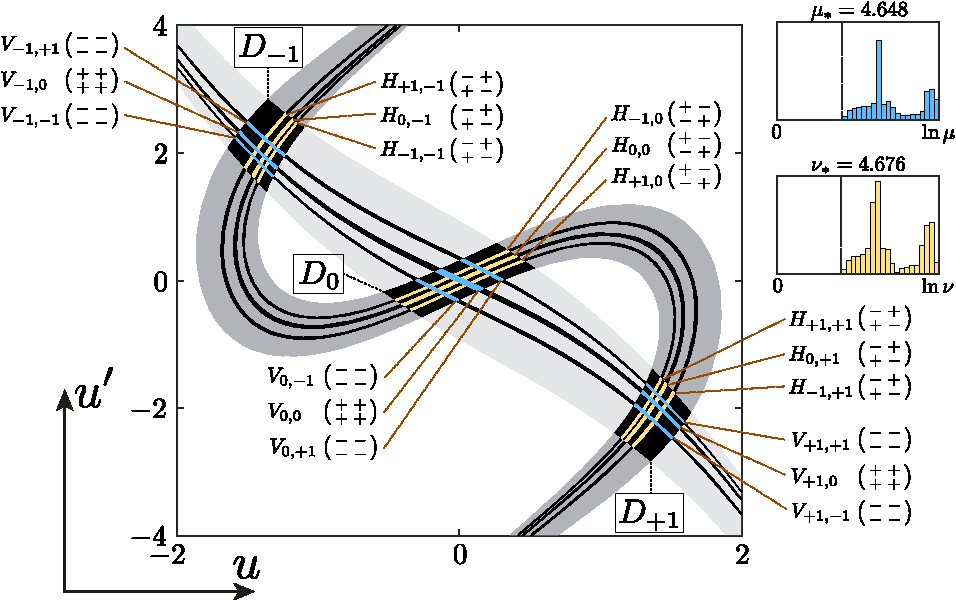
\includegraphics[scale = 1]{pic/hypotheses for piecewise equation}
	\caption{
		Illustration to the verification of Hypothesis~\ref{hypothesis:strips-mapping} for equation \eqref{eq:stationary-piecewise} with parameters $(L_*, L_0) = (2, 1)$ for three-component island set $\mathcal{D}_3 = \{ D_{-1}, D_0, D_{+1} \}$.
	}
\label{fig:hypotheses-validation-piecewise}
\end{figure}

\section{Stationary Solutions of GPE with Piecewise Pseudopotential}

Let's demonstrate how coding of solutions can be used to identify classes of different solutions.
For that purpose we use again Eq.~\eqref{eq:stationary-piecewise} with the parameters $(L_*, L_0) = (2, 1)$.
We have shown previously that there exists a numerical evidence that Hypotheses~\ref{hypothesis:island-set} and \ref{hypothesis:strips-mapping} are valid for three central islands.
We checked them for a lager number of connected component as well, like $5$, $7$, and $9$ central islands, and saw that the hypotheses remain valid.
Let's now restrict our consideration by the first five central components $D_i$, $i \in \{ -2, -1, 0, +1, +2 \}$ of the island set $\mathscr{U}_L$.
Since our numerical analysis shown that both Hypothesis~\ref{hypothesis:island-set} and \ref{hypothesis:strips-mapping} are valid, Theorem~\ref{thm:coding} can be applied.
It allows to conclude that there exists a homeomorphism between a subset of regular solutions and the set $\mathcal{S}_5$.

Such correspondence allows us to make conclusion on different types of regular solutions of equation \eqref{eq:stationary-piecewise}.
For example, there exist periodic solutions of a period $nL$ for any number $n \in \mathbb{N}$.
Their symbolic codes have a periodic structure $\{ \dots, i_0, \dots i_n, i_0, \dots, i_n, \dots \}$.
There also exist localized solutions of different shapes.
Their symbolic codes have a central block of non-zero symbols, and all other symbols on the left and right sides of this block are ``$0$'', $\{ \dots, 0, 0, i_0, \dots, i_n, 0, 0, \dots \}$.
Regular solution of the domain wall shapes can also be found.
They are coded with sequences which has ``$0$'' symbols only on the left or on the right side, $\{ \dots, 0, 0, i_0, i_1, \dots \}$, $\{ \dots, i_{-1}, i_0, 0, 0 \dots \}$.

Several periodic and localized solutions are presented in Figure~\ref{fig:solutions-piecewise}.
Numerical computation of solution by its code in a general case is a separate complex task.
Nevertheless localized solutions can be found by the shooting method, and periodic solutions of a period $nL$ can be found by solving the nonlinear equation $\vb{p} - \mathcal{P}^n(\vb{p}) = 0$, $\vb{p} \in \mathbb{R}^2$, with properly chosen initial approximation which can be guessed from the $\mathscr{U}_L$ structure.
It's worth to mention here the paper \cite{AlfimovKizinZezyulin} where authors provide an algorithm which allows to reconstruct the profile of localized solution by its code for equation \eqref{eq:stationary} with $P(x) \equiv -1$.
Presumably an analogous technique can be applied for a periodic pseudopotential $P(x)$.

% TODO: Take care of this indentation.
\pagebreak
\begin{figure}[h]
\centering
	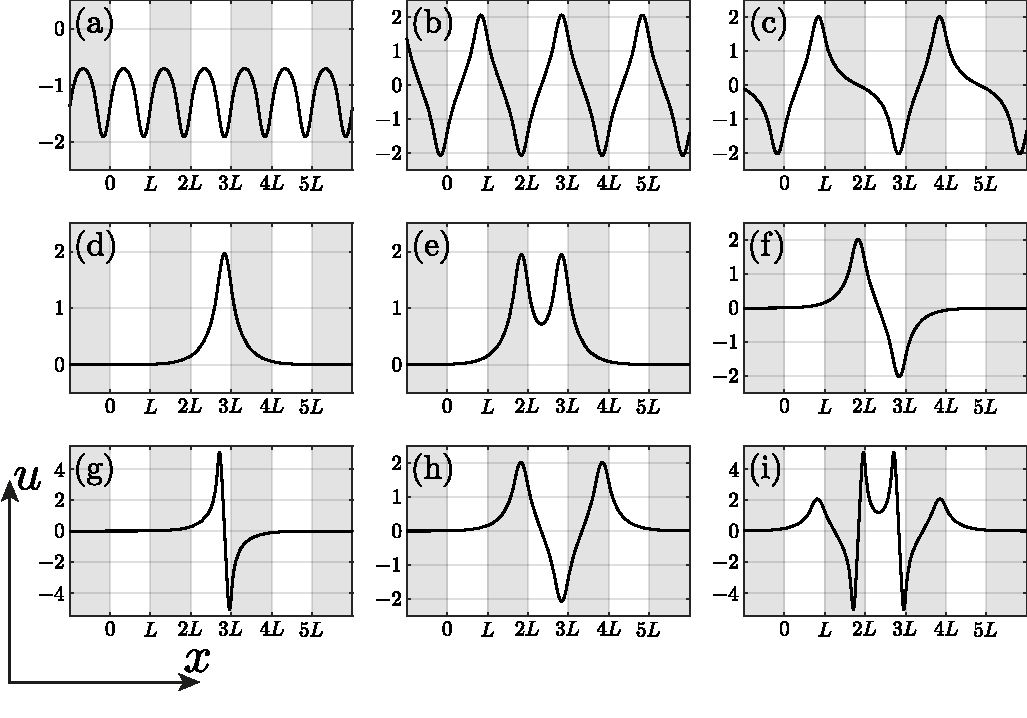
\includegraphics[scale = 1]{pic/solutions for piecewise equation}
	\caption{
		Different solutions for equation \eqref{eq:stationary-piecewise} with parameters $(L_*, L_0) = (2, 1)$.
		Each solution has a corresponding symbolic code, this code identify the solution uniquely.
		Gray strips divide the $x$ axis according to the period $L$.
		First three panels represent periodic solutions, their codes have periodic structure: (a) $L$-periodic solution $\{ \dots, -1, -1, -1, \dots \}$; (b) $2L$-periodic solution $\{ \dots, -1, +1, -1, +1 \dots \}$; (c) $3L$-periodic solution $\{ \dots, -1, +1, 0, -1, +1, 0 \dots \}$.
		Other six panels represent localized solutions, their codes have ``$0$'' symbol to the left and right of the central block: (d) $\{ \dots, 0, 0, +1, 0, 0, \dots \}$; (e) $\{ \dots, 0, 0, +1, +1, 0, 0, \dots \}$ (f) $\{ \dots, 0, 0, +1, -1, 0, 0 \dots \}$ (g) $\{ \dots, 0, 0, -2, 0, 0 \dots \}$ (h) $\{ \dots, 0, 0, +1, -1, +1, 0, 0 \dots \}$ (i) $\{ \dots, 0, 0, +1, +2, -2, +1, 0, 0 \dots \}$.
	}
\label{fig:solutions-piecewise}
\end{figure}

% TODO: Take care of this indentation.
\pagebreak
\section{Summary}

In this chapter the approach for classification of bounded solutions for equation \eqref{eq:stationary} has been exposed.
This approach is based on the analysis of the dynamics of Poincar\'e map $\mathcal{P}$ on the set $\mathscr{U}_L$.
It turns out that under some restrictions the map $\mathcal{P}$ is a horseshoe map with finite or infinite number of partitions.
This allows us to establish a homeomorphism between orbits of regular solutions of \eqref{eq:stationary} and symbolic sequences over some alphabet based on the structure of the set $\mathscr{U}_L$.

We formulated sufficient conditions for the existence of this	 homeomorphism in a form of two hypotheses, see Hypotheses~\ref{hypothesis:island-set} and \ref{hypothesis:strips-mapping}.
Hypothesis~\ref{hypothesis:island-set} can be verified numerically in a straightforward way.
Hypothesis~\ref{hypothesis:strips-mapping} requires a more delicate attitude.
We replaced Hypothesis~\ref{hypothesis:strips-mapping} with Theorems~\ref{thm:h-strips-mapping} and \ref{thm:v-strips-mapping}, they are proved in Appendix~\ref{appendix:strips-mapping-theorems}.
These theorems admits numerical verification by Algorithm~\ref{algorithm:hypotheses-validation}.
If all steps of the algorithm above are successful, we can conclude that Hypothesis~\ref{hypothesis:strips-mapping} takes place. 

The elaborated technique was applied to equation \eqref{eq:stationary-piecewise} with the simplest form of periodic pseudopotential $P(x)$.
On the example of equation \eqref{eq:stationary-piecewise} we show that the presence of sign-altering periodic pseudopotential results in the existence of a plethora of regular solutions.
Such observation allows us we to expect that similar variety of regular solutions is a common property for the overall class of equations \eqref{eq:stationary}.
